\documentclass[11pt,a4paper]{article}
\usepackage[margin=23mm,headheight=14pt,headsep=8.5mm,footskip=10mm]{geometry}
\usepackage{amsmath,amssymb,amsthm}
\usepackage[no-math]{fontspec}
\usepackage{xeCJK}
\setmainfont{Latin Modern Roman}
\setCJKmainfont{FandolSong-Regular.otf}[Script=CustomDefault,Path=assets/fonts/fandol/,BoldFont=FandolSong-Bold.otf,ItalicFont=FandolSong-Regular.otf,BoldItalicFont=FandolSong-Bold.otf]
\setCJKsansfont{FandolSong-Regular.otf}[Script=CustomDefault,Path=assets/fonts/fandol/,BoldFont=FandolSong-Bold.otf]
\xeCJKsetup{PunctStyle=quanjiao,CheckSingle=true}
\usepackage{setspace}
\setstretch{1.12}
\setlength{\parindent}{2em}
\setlength{\parskip}{3pt}
\usepackage{titlesec}
\titleformat{\section}{\centering\normalfont\Large\bfseries}{\thesection.}{0.6em}{}
\titleformat{\subsection}{\normalfont\large\bfseries}{}{0pt}{}
\titlespacing*{\section}{0pt}{1.8\baselineskip}{1.0\baselineskip}
\titlespacing*{\subsection}{0pt}{1.1\baselineskip}{0.5\baselineskip}
\usepackage{enumitem}
\setlist[enumerate]{leftmargin=2em,labelsep=0.5em,itemsep=3pt,parsep=0pt,topsep=6pt}
\providecommand{\tightlist}{\setlength{\itemsep}{3pt}\setlength{\parskip}{0pt}}
\usepackage{needspace}
\newenvironment{statementblock}{\par\Needspace{9\baselineskip}\noindent}{\par\nopagebreak[4]}
\newenvironment{proofblock}{\par\Needspace{4\baselineskip}\noindent}{\par}
\usepackage{fancyhdr}
\pagestyle{fancy}
\fancyhf{}
\fancyhead[L]{\small 数学手记}
\fancyhead[R]{\small 复变函数 · 第五章}
\fancyfoot[C]{\thepage}
\renewcommand{\headrulewidth}{0.4pt}
\usepackage[hidelinks,unicode,bookmarksnumbered=true,linktoc=all]{hyperref}
\usepackage{bookmark}
\bookmarksetup{depth=2}
\hypersetup{pdftitle={复变函数讲义：第五章},pdfauthor={Vincent Arqain},pdfsubject={全纯函数的 Laurent 展开及其应用}}
\renewcommand{\contentsname}{目录}
\setcounter{tocdepth}{1}
\setcounter{secnumdepth}{1}
\widowpenalty=10000
\clubpenalty=10000
\displaywidowpenalty=10000
\predisplaypenalty=10000
\interdisplaylinepenalty=10000
\raggedbottom

\usepackage{tabularx,booktabs,array}
\renewcommand{\thesection}{5.\arabic{section}}
\emergencystretch=2em

\usepackage{graphicx}
\usepackage{longtable}
\usepackage{calc}
\usepackage{float}
\floatplacement{figure}{H}
\renewcommand{\figurename}{图}
\makeatletter
\def\maxwidth{\ifdim\Gin@nat@width>\linewidth\linewidth\else\Gin@nat@width\fi}
\def\maxheight{\ifdim\Gin@nat@height>0.72\textheight0.72\textheight\else\Gin@nat@height\fi}
\makeatother
\setkeys{Gin}{width=\maxwidth,height=\maxheight,keepaspectratio}
\providecommand{\pandocbounded}[1]{#1}
\setcounter{tocdepth}{2}
\begin{document}
\begin{center}
{\LARGE\bfseries 复变函数讲义\par}
\vspace{8pt}{\large 第五章\quad 全纯函数的 Laurent 展开及其应用\par}
\vspace{6pt}{\small 依史济怀、刘太顺《复变函数》\quad 教材第 141—193 页\par}
\end{center}\vspace{8pt}
本章含7节讲义及全部 58 道习题原题。定义、定理和性质沿用教材的记号与编号；证明补足必要条件、退化情形与关键推导。覆盖 54 个教材编号条目，补证 Picard 大定理，逐项说明积分的主值、分支与收敛条件；给出 Mittag–Leffler、零点构造、插值及 Blaschke 乘积的证明。58 道主编号题中含 31 个积分小题，保留教材围道图及提示。习题不附解答，原题中的疑义另列校勘。
\tableofcontents\clearpage
\section{全纯函数的 Laurent 展开}
对应教材第 141---146 页。Taylor 展开研究圆盘；Laurent
展开研究圆环。两条边界给出两种几何级数，正幂记录外边界，负幂记录内边界。本章沿用
\(H(D)\)、\(B(a,r)\)、\(\mathbb C_\infty\) 与
\(\operatorname{Res}(f,a)\)；\(B(\infty,R)\) 表示 \(|z|>R\)
的有限点部分，无穷远点的性质通过 \(w=1/z\) 定义。

\Needspace{5\baselineskip}
\subsection{Laurent 级数与收敛圆环}\label{ch05-s1-heading-1}

Laurent 级数是

\[
\sum_{n=-\infty}^{\infty}a_n(z-z_0)^n
=\sum_{n=0}^{\infty}a_n(z-z_0)^n+\sum_{n=1}^{\infty}a_{-n}(z-z_0)^{-n}.
\qquad\text{(5.1.1)}
\]

其收敛指右边两个级数分别收敛，不采用对称部分和定义。前者为全纯部分，后者为主要部分。设正幂级数半径为
\(R\)，而 \(\sum_{n\ge1}a_{-n}w^n\) 的半径为 \(\rho\)，令
\(r=1/\rho\)，约定 \(1/0=\infty\)、\(1/\infty=0\)。共同的开收敛区域为
\(r<|z-z_0|<R\)。

\textbf{定理 5.1.1。} 若 \(r<R\)，式（5.1.1）在圆环
\(D=\{r<|z-z_0|<R\}\) 中绝对且内闭一致收敛，其和属于 \(H(D)\)。

证明：任取紧集 \(K\subset D\)，存在 \(r<r_1\le|z-z_0|\le r_2<R\) 覆盖
\(K\)。正幂项由半径 \(r_2\) 处的绝对收敛级数控制，负幂项作
\(w=(z-z_0)^{-1}\) 后由半径 \(1/r_1<\rho\)
处的绝对收敛级数控制。两部分均满足 Weierstrass 判别法；各项在 \(D\)
全纯，再用定理 4.1.9。

当 \(R<r\) 时不存在共同收敛点；当 \(R=r>0\)
时没有开收敛圆环，但圆周上的共同收敛仍可能发生。例如
\(a_n=1/n^2\)、\(a_{-n}=1/n^2\)（\(n\ge1\)），\(a_0=0\)，两部分在
\(|z-z_0|=1\) 均绝对收敛。教材``\(R\le r\)
时两者不能同时收敛''须作这一边界修正。

\Needspace{5\baselineskip}
\subsection{定理 5.1.2：存在性、系数与唯一性}\label{ch05-s1-heading-2}

设 \(f\in H(D)\)，\(D=\{r<|z-z_0|<R\}\)。则

\[
\begin{aligned}
f(z)&=\sum_{n=-\infty}^{\infty}a_n(z-z_0)^n,\\
a_n&=\frac1{2\pi i}\int_{\gamma_\rho}\frac{f(\zeta)}{(\zeta-z_0)^{n+1}}\,d\zeta,
\quad n\in\mathbb Z,
\end{aligned}
\qquad\text{(5.1.2)}
\]

其中 \(r<\rho<R\)，\(\gamma_\rho\) 为正向圆周
\(|\zeta-z_0|=\rho\)。展开在 \(D\) 内闭绝对一致，且唯一；系数不依赖
\(\rho\)。

证明：固定 \(z\in D\)，选 \(r<r_1<|z-z_0|<r_2<R\)。由多连通 Cauchy
公式，外圆、内圆均取逆时针方向时，

\[
f(z)=\frac1{2\pi i}\int_{\gamma_{r_2}}\frac{f(\zeta)}{\zeta-z}\,d\zeta
-\frac1{2\pi i}\int_{\gamma_{r_1}}\frac{f(\zeta)}{\zeta-z}\,d\zeta.
\qquad\text{(5.1.3)}
\]

分别展开

\[
\begin{aligned}
\frac1{\zeta-z}&=\sum_{n=0}^{\infty}\frac{(z-z_0)^n}{(\zeta-z_0)^{n+1}}
&&(|\zeta-z_0|=r_2),\\
\frac1{\zeta-z}&=-\sum_{n=1}^{\infty}\frac{(\zeta-z_0)^{n-1}}{(z-z_0)^n}
&&(|\zeta-z_0|=r_1).
\end{aligned}
\]

几何比的模分别为
\(|z-z_0|/r_2<1\)、\(r_1/|z-z_0|<1\)，故在积分圆周上一致收敛，可逐项积分。对任意整数
\(n\)，函数 \(f(\zeta)/(\zeta-z_0)^{n+1}\) 在两圆之间全纯，多连通 Cauchy
定理说明系数积分不依赖半径，遂得（5.1.2）。对紧集先选统一的内外辅助圆，以上两个几何比便一致小于
\(1\)，同时得到内闭绝对一致收敛。

若另有系数 \(b_n\)，在任一 \(\gamma_\rho\) 上逐项积分，利用

\[
\frac1{2\pi i}\int_{\gamma_\rho}(\zeta-z_0)^{n-m-1}\,d\zeta
=\begin{cases}1,&n=m,\\0,&n\ne m,\end{cases}
\]

得
\(b_m=a_m\)。正、负两部分都在圆周上一致收敛，这正是交换求和与积分的依据。

\textbf{系数估计。} 若 \(M(\rho)=\max_{\gamma_\rho}|f|\)，长大不等式给出
\(|a_n|\le M(\rho)\rho^{-n}\)（\(n\in\mathbb Z\)）。特别地，\(|a_{-n}|\le M(\rho)\rho^n\)，这是可去奇点定理的关键。

\textbf{求导与积分。} 由定理 4.1.9，Laurent
级数可在圆环内逐项求任意固定阶导数。它在整个圆环有单值原函数，当且仅当
\(a_{-1}=0\)。必要性由闭圆周积分为
\(2\pi i a_{-1}\)；充分性将其余各项积成
\(a_n(z-z_0)^{n+1}/(n+1)\)。对紧子圆环取稍大的两边界，几何级数估计仍保证所得级数内闭一致收敛，逐项求导即回到
\(f\)。

\Needspace{5\baselineskip}
\subsection{例 5.1.3：同一函数的不同圆环}\label{ch05-s1-heading-3}

对 \(f(z)=1/[(z-1)(z-2)]\)，先拆成 \(1/(z-2)-1/(z-1)\)。因此

\[
\begin{aligned}
f(z)&=-\sum_{n=0}^{\infty}\frac{z^n}{2^{n+1}}-\sum_{n=1}^{\infty}z^{-n},&&1<|z|<2,\\
f(z)&=\sum_{n=0}^{\infty}(2^n-1)z^{-n-1},&&2<|z|<\infty.
\end{aligned}
\]

每一步都将分母改成几何比模小于 \(1\)
的形式。两式不矛盾：唯一性必须同时固定中心和圆环；跨过极点后，系数积分不能再用
Cauchy 定理相互移动。

\Needspace{5\baselineskip}
\subsection{本节索引}\label{ch05-s1-heading-4}

\hyperref[ch05-s1-heading-1]{Laurent 级数与收敛圆环} · \hyperref[ch05-s1-heading-2]{定理
5.1.2：存在性、系数与唯一性} · \hyperref[ch05-s1-heading-3]{例
5.1.3：同一函数的不同圆环}

\section{孤立奇点}
对应教材第 146---151 页。奇点分类由 Laurent 主要部分决定。教材略去的
Picard
大定理在本节另给完整补证；只使用前三、四章及实分析中的紧性，不预先借用第七章。

\Needspace{5\baselineskip}
\subsection{可去奇点、极点与本性奇点}\label{ch05-s2-heading-1}

若 \(f\) 在 \(0<|z-z_0|<R\) 全纯，称 \(z_0\)
为孤立奇点。极限为有限值时称可去奇点，球面极限为 \(\infty\)
时称极点，球面极限不存在时称本性奇点。

\textbf{定理 5.2.1（Riemann）。} 孤立奇点 \(z_0\) 可去，当且仅当 \(f\)
在某个无心邻域有界。

证明：有限极限必使 \(f\) 局部有界。反之，设
\(|f|\le M\)；由（5.1.2）对每个 \(n\ge1\) 得 \(|a_{-n}|\le M\rho^n\)。令
\(\rho\downarrow0\)，得全部负幂系数为零。因此 \(f\) 是幂级数的限制，定义
\(f(z_0)=a_0\) 就得到全纯延拓。延拓唯一，因为连续性确定了该值。

\textbf{命题 5.2.2。} \(z_0\) 是 \(f\) 的极点，当且仅当 \(1/f\)
在足够小的无心邻域有定义，并全纯延拓为以 \(z_0\) 为零点的函数。

证明：\(f(z)\to\infty\) 使 \(f\) 最终非零且
\(1/f\to0\)，用可去奇点定理。反向由 \(1/f\to0\) 且在无心邻域非零得到
\(|f|\to\infty\)。

\textbf{定义 5.2.3。} 若延拓后的 \(1/f\) 在 \(z_0\) 有 \(m\) 阶零点，称
\(z_0\) 为 \(f\) 的 \(m\) 阶极点。

\textbf{定理 5.2.4。} \(z_0\) 为 \(m\) 阶极点，当且仅当

\[
f(z)=\frac{a_{-m}}{(z-z_0)^m}+\cdots+\frac{a_{-1}}{z-z_0}
+\sum_{n=0}^{\infty}a_n(z-z_0)^n,\qquad a_{-m}\ne0.
\qquad\text{(5.2.2)}
\]

证明：由零点分解 \(1/f=(z-z_0)^m g\)，\(g(z_0)\ne0\)，将 \(1/g\) 展成
Taylor 级数即可。反之，（5.2.2）使 \(h=(z-z_0)^m f\) 全纯且
\(h(z_0)=a_{-m}\ne0\)，故 \(1/f=(z-z_0)^m/h\) 有恰好 \(m\) 阶零点。

于是三类奇点的主要部分分别为：没有负幂项、有限个非零负幂项、无穷多个非零负幂项。第三类由前两类的充要条件和分类定义立即得到；``本性''不是``极点阶数无限大''的代数运算。

\Needspace{5\baselineskip}
\subsection{定理 5.2.5：本性奇点的值域稠密}\label{ch05-s2-heading-2}

若 \(z_0\) 为本性奇点，则对每个 \(A\in\mathbb C_\infty\)，存在
\(z_n\to z_0\)、\(z_n\ne z_0\)，使 \(f(z_n)\to A\)。

证明：每个无心邻域内 \(f\) 都无界，否则奇点可去；故可取
\(0<|z_n-z_0|<1/n\)、\(|f(z_n)|>n\)，得到 \(A=\infty\)。若有限值 \(A\)
不能被这样逼近，则某无心邻域上 \(|f-A|\ge\varepsilon>0\)。此时
\(g=1/(f-A)\) 才确实全纯且有界，可延拓至 \(z_0\)。若
\(g(z_0)\ne0\)，\(f=A+1/g\) 可去；若 \(g(z_0)=0\)，\(g\)
不恒零，由零点有限阶分解知 \(f\) 有极点，均矛盾。不能在尚未排除 \(f=A\)
时直接宣称 \(1/(f-A)\) 在整个无心邻域全纯。

\Needspace{5\baselineskip}
\subsection{定理 5.2.6：Picard 大定理}\label{ch05-s2-heading-3}

全纯函数在本性孤立奇点的每个无心邻域内，无穷多次取到每个有限复值，至多有一个例外。

下面补证``省略两个值的全纯函数不能有本性孤立奇点''。辅助的密度估计只是一条二维微分不等式，不需要先接受双曲几何理论。

\textbf{补充引理 A（一个显式密度）。} 在
\(\Omega=\mathbb C\setminus\{0,1\}\) 上存在正的 \(C^2\) 函数 \(\lambda\)
和常数 \(c>0\)，使

\[
\Delta\log\lambda\ge\lambda^2,
\qquad \lambda(w)\ge\frac{c}{1+|w|^2},
\quad \Delta=\partial_x^2+\partial_y^2.
\qquad\text{(补5.2-A)}
\]

证明：令 \(p=1/4\)、\(a=7/8\)，并取

\[
\lambda_0(w)=\frac{(1+|w|^p)(1+|w-1|^p)}{|w|^a|w-1|^a}.
\]

\(\log|w|\)、\(\log|w-1|\) 在 \(\Omega\) 调和，径向求导给出

\[
\Delta\log\lambda_0
=p^2\left[\frac{|w|^{p-2}}{(1+|w|^p)^2}
+\frac{|w-1|^{p-2}}{(1+|w-1|^p)^2}\right]>0.
\]

记 \(Q=(\Delta\log\lambda_0)/\lambda_0^2\)。当 \(w\to0\) 或 \(1\)
时，\(Q\to1/64\)；当 \(|w|\to\infty\)
时，\(Q\sim |w|^{1/4}/8\to\infty\)。删去这三个端点邻域后是紧集，\(Q\)
连续为正，故 \(k=\inf_\Omega Q>0\)。取 \(\lambda=\sqrt{k}\lambda_0\)
即有第一式。又 \(\lambda_0(1+|w|^2)\) 在 \(0,1,\infty\)
均趋无穷，紧集上有正最小值，第二式成立。

\textbf{补充引理 B（圆盘上的导数控制）。} 若 \(F:B(0,R)\to\Omega\)
全纯，则

\[
\lambda(F(z))|F'(z)|\le\frac{2R}{R^2-|z|^2}.
\qquad\text{(补5.2-B)}
\]

证明：固定 \(r<R\)，记
\(\sigma=\lambda(F)|F'|\)、\(v_r=2r/(r^2-|z|^2)\)。若 \(F\) 非常数，在
\(F'\ne0\) 处用链式法则及 \(\log|F'|\) 调和，得
\(\Delta\log\sigma\ge\sigma^2\)；直接求导得
\(\Delta\log v_r=v_r^2\)。\(\sigma\) 在闭盘 \(|z|\le r\) 有界，而
\(v_r\) 在边界趋无穷，故 \(\sigma/v_r\)
的正最大值在内部取得。若最大值大于 \(1\)，该点 \(\sigma>0\)，则
\(\Delta\log(\sigma/v_r)\ge\sigma^2-v_r^2>0\)，与内部极大值处的
Laplacian 非正矛盾。故 \(\sigma\le v_r\)；令
\(r\uparrow R\)。常函数情形左端为零。临界点处不取对数，因此没有除零问题。

\textbf{补充引理 C（省略两个值的紧性）。} 任意一列省略 \(0,1\)
的全纯函数，在域内有子列按球面距离内闭一致收敛，极限为亚纯函数或恒等于
\(\infty\)。

证明：用（补5.2-A、B）在每个内含圆盘控制球面导数
\(|F'|/(1+|F|^2)\)。沿小线段积分，得到球面距离下的局部等度连续。球面紧，由
Arzelà--Ascoli
定理及可数紧集穷竭的对角选取，得到球面局部一致极限。为核实极限的解析性，在每点选择一个不含极限值的球面点；连续性保证一个小盘上的极限像及最终的函数像都避开该点的固定邻域。把该点用分式线性变换移至无穷远，便化为有界全纯函数的普通局部一致收敛，Weierstrass
定理给出极限全纯。反变换说明极限是球面值全纯映射；若不恒为无穷远，它即为亚纯函数。

还需一个细节：若这一极限在某点为有限非零值，则极限没有极点。否则在极点的小圆盘上，\(1/F_n\)
普通一致收敛于 \(1/F\)；后者在中心为零且不恒零，而 \(1/F_n\)
无零点，与第四章 Hurwitz
定理矛盾。连通性排除了在某开集恒为无穷远、另一处有限的情形。同理，非恒零的有限极限不取
\(0\)；对 \(F_n-1\) 可知也不取 \(1\)。

\textbf{Picard 定理的证明。} 平移奇点到 \(0\)。若 \(f\)
在某无心盘省略两个不同有限值，作仿射变换可设省略 \(0,1\)。假设 \(0\)
本性，由定理 5.2.5 取 \(z_n\to0\)、\(f(z_n)\to2\)。令
\(F_n(w)=f(z_n w)\)，其定义域最终包含 \(\mathbb C\setminus\{0\}\)
的每个紧集。引理 C 的对角选取得到球面内闭一致极限 \(F\)；因
\(F(1)=2\)，上面的细节说明 \(F\) 在 \(\mathbb C\setminus\{0\}\) 全纯。故
\(F_n\) 在 \(|w|=1\) 上最终有统一的普通模界 \(M\)。

于是 \(|f(z)|\le M\) 于圆周
\(|z|=|z_n|\)。选取模严格递减的子列；对相邻圆周之间的闭圆环用最大模原理，得到整个足够小无心盘内
\(|f|\le M\)。Riemann
定理说明奇点可去，矛盾。因此本性奇点邻域不能省略两个有限值。若两个值在某邻域各只取有限次，再缩小邻域排除这些有限个原像，就省略了两个值，同样矛盾。这也证明了``无穷多次''的完整结论。

例如 \(e^{1/z}\) 的例外值为 \(0\)；对任意 \(A\ne0\)，固定一支
\(\log A\)，取
\(z_n=(\log A+2\pi i n)^{-1}\)（略去可能使分母为零的一项），则
\(z_n\to0\) 且 \(e^{1/z_n}=A\)。

\Needspace{5\baselineskip}
\subsection{定义 5.2.7：无穷远点}\label{ch05-s2-heading-4}

若 \(f\) 在 \(|z|>R\) 全纯，令 \(g(w)=f(1/w)\)，以 \(g\) 在 \(0\)
的性质定义 \(f\) 在 \(\infty\) 的可去奇点、\(m\) 阶极点与本性奇点。

若 \(g(w)=\sum a_nw^n\)，则
\(f(z)=\sum a_{-n}z^n\)。因此在无穷远点，全纯部分为
\(b_0+\sum_{n\ge1}b_{-n}z^{-n}\)，主要部分为
\(\sum_{n\ge1}b_nz^n\)。可去、\(m\)
阶极点、本性分别对应正幂项全无、最高正幂恰为
\(m\)、无穷多个非零正幂项。教材（5.2.4）的 \(b_1\) 项应为 \(b_1z\)。

``无穷远处有无穷多极点''不属于孤立奇点：此时任意外部区域都有极点，无法对
\(f(1/w)\) 在一个完整无心盘作上述分类。

\Needspace{5\baselineskip}
\subsection{本节索引}\label{ch05-s2-heading-5}

\hyperref[ch05-s2-heading-1]{可去奇点、极点与本性奇点} ·
\hyperref[ch05-s2-heading-2]{定理 5.2.5：本性奇点的值域稠密} ·
\hyperref[ch05-s2-heading-3]{定理 5.2.6：Picard 大定理} ·
\hyperref[ch05-s2-heading-4]{定义 5.2.7：无穷远点}

\section{整函数与亚纯函数}
对应教材第 151---154
页。整函数和有理函数可以通过无穷远点识别：有限平面的局部信息与球面的紧性共同给出全局分类。

\Needspace{5\baselineskip}
\subsection{整函数在无穷远点的三种情形}\label{ch05-s3-heading-1}

\textbf{定理 5.3.1。} 在无穷远点全纯的整函数一定是常数。

证明：整函数有全平面 Taylor 展开
\(f(z)=\sum_{n\ge0}a_nz^n\)。无穷远点可去时，在外部圆环的 Laurent
展开没有正幂项。由唯一性
\(a_n=0\)（\(n\ge1\)），故为常数。也可用外部有界性和内部紧性得到全平面有界，再用
Liouville 定理。

\textbf{定理 5.3.2。} 无穷远点为整函数 \(f\) 的 \(m\) 阶极点，当且仅当
\(f\) 是恰好 \(m\) 次多项式。

证明：外部 Laurent 展开最高正幂为 \(m\) 且系数非零，与全平面 Taylor
展开比较即可。反之 \(f(1/w)=w^{-m}(a_m+a_{m-1}w+\cdots+a_0w^m)\)，括号在
\(0\) 非零。

不是多项式的整函数称超越整函数。其无穷远点必为本性奇点，因为前两种情形已经穷尽多项式。\(e^z,\sin z,\cos z\)
均属此类。

\Needspace{5\baselineskip}
\subsection{定理 5.3.3：球面亚纯函数即有理函数}\label{ch05-s3-heading-2}

亚纯函数在每个有限点附近或者全纯，或者具有有限阶极点；不将恒等于
\(\infty\) 纳入通常的亚纯函数域。若 \(\infty\) 是平面亚纯函数 \(f\)
的可去奇点或极点，则 \(f\) 是有理函数。

证明：\(f\) 在某 \(|z|>R\)
无有限极点。闭盘中极点若无限，紧性给出有限聚点，与该点附近全纯或只有一个极点矛盾。因此有限极点只有
\(z_1,\ldots,z_N\)。记 \(h_j\) 为各点的有限 Laurent 主要部分，\(g\)
为无穷远处的主要部分（多项式，且常数项取零）。则

\[
F=f-g-\sum_{j=1}^N h_j
\]

在每个有限极点的主要部分被抵消，因而延拓为整函数；在无穷远处也可去。由定理
5.3.1，\(F=c\)，即

\[
f(z)=c+g(z)+\sum_{j=1}^N h_j(z).
\]

反之，既约有理函数 \(P_n/Q_m\) 在无穷远处，若 \(n>m\) 为 \(n-m\)
阶极点；若 \(n=m\) 可去且值为首项系数比；若 \(n<m\) 可去且有 \(m-n\)
阶零点。这由分子分母除以各自最高幂直接得到。

\textbf{部分分式唯一性。} 对同一有理函数，各有限极点的主要部分由 Laurent
唯一性确定；相减后剩余多项式也唯一。上述论证同时给出存在性与唯一性。

\Needspace{5\baselineskip}
\subsection{平面与球面的自同构}\label{ch05-s3-heading-3}

\textbf{定理 5.3.4。} \(\operatorname{Aut}(\mathbb C)=\{az+b:a\ne0\}\)。

证明：线性函数显然有全纯反函数。反之，若双全纯映射
\(f:\mathbb C\to\mathbb C\) 在无穷远处可去，则为常数；若本性，由定理
5.2.5 可取
\(z_n\to\infty\)、\(f(z_n)\to A\in\mathbb C\)。反函数连续性给出
\(z_n=f^{-1}(f(z_n))\to f^{-1}(A)\)，矛盾。故 \(f\)
是多项式。单叶全纯函数的导数处处非零；若次数至少 \(2\)，\(f'\)
是非常数多项式，由代数基本定理必有零点，矛盾。

\textbf{定理 5.3.5。} \(\operatorname{Aut}(\mathbb C_\infty)\)
恰为分式线性变换 \(f(z)=(az+b)/(cz+d)\)，其中 \(ad-bc\ne0\)。

证明：分式线性变换在球面有同类反变换。反之，取球面双全纯映射
\(f\)，以分式线性变换 \(T\) 将唯一的 \(f(\infty)\) 移至 \(\infty\)。于是
\(T\circ f\) 只在 \(\infty\) 取无穷值，其有限平面限制是 \(\mathbb C\)
的双全纯自同构，故为一次多项式。于是 \(f=T^{-1}\circ(az+b)\)
是分式线性变换。这里在球面坐标下始终说全纯映射，不能将有限值函数在极点处的发散误认为球面映射不连续。

\Needspace{5\baselineskip}
\subsection{本节索引}\label{ch05-s3-heading-4}

\hyperref[ch05-s3-heading-1]{整函数在无穷远点的三种情形} ·
\hyperref[ch05-s3-heading-2]{定理 5.3.3：球面亚纯函数即有理函数} ·
\hyperref[ch05-s3-heading-3]{平面与球面的自同构}

\section{残数定理}
对应教材第 154---161 页。残数抽取 Laurent 展开的 \(-1\)
次系数；积分的拓扑信息由绕数承担。全节闭曲线默认正向，复合边界为外边界逆时针、内边界顺时针。

\Needspace{5\baselineskip}
\subsection{定义 5.4.1 与无穷远点的符号}\label{ch05-s4-heading-1}

若 \(a\) 为孤立奇点，\(f(z)=\sum c_n(z-a)^n\)，定义
\(\operatorname{Res}(f,a)=c_{-1}\)。故对足够小的正向圆周 \(\gamma\)，

\[
\int_\gamma f(z)\,dz=2\pi i\operatorname{Res}(f,a).
\qquad\text{(5.4.2)}
\]

证明：在圆周上逐项积分；除 \(n=-1\)
外各项积分为零。对无心盘中任意闭曲线应乘绕数
\(\operatorname{Ind}(\gamma,a)\)，并非任何闭曲线的积分都相等。例如绕两周便得到两倍积分。

若 \(f\) 在 \(|z|>R\) 全纯，定义

\[
\operatorname{Res}(f,\infty)=-\frac1{2\pi i}\int_{|z|=\rho}f(z)\,dz,
\qquad \rho>R.
\qquad\text{(5.4.3)}
\]

它是外部 Laurent 展开中 \(z^{-1}\) 系数的相反数。作
\(z=1/w\)，\(dz=-w^{-2}dw\)，得

\[
\operatorname{Res}(f,\infty)
=\operatorname{Res}\left(-\frac{f(1/w)}{w^2},0\right).
\qquad\text{(补5.4-A)}
\]

残数变换的是微分 \(f(z)\,dz\)，不是仅将函数换成 \(f(1/w)\)。例如 \(1/z\)
在 \(\infty\) 可去，但其无穷远残数为 \(-1\)。

\Needspace{5\baselineskip}
\subsection{极点残数的计算}\label{ch05-s4-heading-2}

\textbf{命题 5.4.2。} 若 \(a\) 为 \(m\) 阶极点，令 \(g(z)=(z-a)^mf(z)\)
在 \(a\) 处按可去方式补值，则

\[
\operatorname{Res}(f,a)=\frac{g^{(m-1)}(a)}{(m-1)!}
=\frac1{(m-1)!}\lim_{z\to a}\frac{d^{m-1}}{dz^{m-1}}[(z-a)^mf(z)].
\]

证明：展开 \(g=\sum g^{(n)}(a)(z-a)^n/n!\)，乘 \((z-a)^{-m}\)；\(-1\)
次项来自 \(n=m-1\)。

\textbf{命题 5.4.3。} 一阶极点时
\(\operatorname{Res}(f,a)=\lim_{z\to a}(z-a)f(z)\)，即上一命题的 \(m=1\)
情形。

\textbf{例 5.4.4。} \(f(z)=1/(1+z^2)\) 在 \(\pm i\) 的残数分别为
\(1/(2i)\)、\(-1/(2i)\)，因为约去相应一次因子后，余下因子在该点的值为
\(\pm2i\)。

\textbf{命题 5.4.5。} 若 \(g,h\) 在 \(a\)
全纯，\(g(a)\ne0\)、\(h(a)=0\)、\(h'(a)\ne0\)，则 \(g/h\) 在 \(a\)
为一阶极点，且残数为 \(g(a)/h'(a)\)。

证明：\(h(z)/(z-a)\to h'(a)\ne0\)，在命题 5.4.3 中取极限即可。

\textbf{例 5.4.6。} \(e^z/\sin z\) 在 \(0\) 的残数为 \(e^0/\cos0=1\)。

\textbf{例 5.4.7。} 对 \(f(z)=e^{iz}/[z(z^2+1)^2]\)，\(-i\)
为二阶极点。令 \(g(z)=e^{iz}/[z(z-i)^2]\)，则 \(g(-i)=e/(4i)\)，且

\[
\frac{g'(z)}{g(z)}=i-\frac1z-\frac2{z-i},
\qquad g'(-i)=\frac e{4i}(-i)=-\frac e4.
\]

因此残数为 \(-e/4\)。教材写 \(e/4\)，漏了负号；这一处已直接微分复核。

\textbf{例 5.4.8。} \(e^{z+1/z}\) 在 \(0\)
本性；在任一固定圆周上，两指数级数绝对一致，允许乘积求和。指数
\(k-j=-1\) 给出

\[
\operatorname{Res}(e^{z+1/z},0)=\sum_{k=0}^{\infty}\frac1{k!(k+1)!}.
\]

\Needspace{5\baselineskip}
\subsection{定理 5.4.9：残数定理}\label{ch05-s4-heading-3}

设 \(D\) 为有界域，边界由有限条可求长简单闭曲线组成；\(f\) 在 \(D\)
除有限个孤立奇点 \(z_1,\ldots,z_N\) 外全纯，并连续到其余闭域。则

\[
\int_{\partial D}f(z)\,dz=2\pi i\sum_{k=1}^N\operatorname{Res}(f,z_k).
\qquad\text{(5.4.5)}
\]

证明：在每个 \(z_k\) 周围取互不相交且闭包在 \(D\) 内的小圆盘。从 \(D\)
挖去这些圆盘后，\(f\) 全纯，第三章的多连通 Cauchy
定理给出外复合边界积分等于各小圆的逆时针积分之和。逐个应用（5.4.2）即得。可求长边界的连续到边界版本使用第三章已证的边界逼近结论；不能仅凭示意图把任意闭曲线当作正向简单边界。

\textbf{带绕数形式。} 若闭曲线 \(\gamma\)
在域内零调且不经过奇点，则其积分为
\(2\pi i\sum\operatorname{Ind}(\gamma,z_k)\operatorname{Res}(f,z_k)\)。对每个孤立奇点取完整的
Laurent
主要部分（允许无穷多项）；该负幂级数在除该点以外的整个平面全纯，因为把它视为
\(1/(z-a)\) 的幂级数时收敛半径无穷。扣除所涉及的有限个主部后，用零调
Cauchy 定理；每个主部在曲线上一致收敛，可逐项积分，仅 \(-1\)
次项留下相应绕数。后文单连通域中的闭路径正是这一情形。

\Needspace{5\baselineskip}
\subsection{例 5.4.10---5.4.11}\label{ch05-s4-heading-4}

\textbf{例 5.4.10。} 在 \(|z-1|=\sqrt3\) 内，\(z/[(z^2-1)^2(z^2+1)]\)
的极点为 \(i,-i,1\)，\(-1\) 在外。前两点残数均为 \(1/8\)；在 \(1\) 处对
\(z/[(z+1)^2(z^2+1)]\) 求导，得 \(-1/8\)。因此积分为
\(2\pi i(1/8+1/8-1/8)=\pi i/4\)。

\textbf{例 5.4.11。} 在 \(|z|<1\) 中，\(z^2\sin^2z/(1-e^z)^5\) 仅在
\(0\) 有极点。因 \(\sin z=z+O(z^3)\)、\(1-e^z=-z+O(z^2)\)，故

\[
\frac{z^2\sin^2z}{(1-e^z)^5}=-\frac1z(1+O(z)),
\qquad \int_{|z|=1}\frac{z^2\sin^2z}{(1-e^z)^5}\,dz=-2\pi i.
\]

\Needspace{5\baselineskip}
\subsection{定理 5.4.12：包括无穷远点的残数和}\label{ch05-s4-heading-5}

若 \(f\) 在 \(\mathbb C\)
除有限个孤立奇点外全纯，则这些有限奇点与无穷远点的残数总和为零。

证明：取包含所有有限奇点的大圆，残数定理给出圆周积分为有限残数和的
\(2\pi i\) 倍；（5.4.3）给出同一积分为无穷远残数的 \(-2\pi i\)
倍。这里允许有限点或无穷远点为本性奇点，不限于有理函数。

\textbf{对数导数与零极点计数。} 若
\(f=(z-a)^m h\)、\(h(a)\ne0\)，其中整数 \(m\)
正值表示零点、负值表示极点，则 \(f'/f=m/(z-a)+h'/h\)，残数为 \(m\)。故
\(\int f'/f\)
计数``零点总阶减极点总阶''。这一结论解释了第四章辐角原理的亚纯推广；边界上必须既无零点又无极点。

\Needspace{5\baselineskip}
\subsection{本节索引}\label{ch05-s4-heading-6}

\hyperref[ch05-s4-heading-1]{定义 5.4.1 与无穷远点的符号} ·
\hyperref[ch05-s4-heading-2]{极点残数的计算} · \hyperref[ch05-s4-heading-3]{定理
5.4.9：残数定理} · \hyperref[ch05-s4-heading-4]{例 5.4.10---5.4.11} ·
\hyperref[ch05-s4-heading-5]{定理 5.4.12：包括无穷远点的残数和}

\section{利用残数定理计算定积分}
教材第 161---179
页。本节所有围道均按区域在左侧的方向取正向；半圆凹口因而沿顺时针方向绕过实轴上的奇点。先判断积分是否存在，再用残数计算数值。

\Needspace{5\baselineskip}
\subsection{定理 5.5.1、推论 5.5.2：上半平面有理型积分}\label{ch05-s5-heading-1}

设 \(f\) 在闭上半平面的一个邻域内，除上半平面中有限个孤立奇点
\(a_1,\ldots,a_n\) 外全纯，实轴上无奇点，且 \(zf(z)\to0\) 在上半平面内随
\(|z|\to\infty\) 一致成立。则

\[
\operatorname{PV}\int_{-\infty}^{\infty}f(x)\,dx
=2\pi i\sum_{k=1}^n\operatorname{Res}(f,a_k).
\qquad\text{(5.5-A)}
\]

这里 \(\operatorname{PV}\) 表示
\(\lim_{R\to\infty}\int_{-R}^R\)；若左右两个反常积分分别存在，就可去掉主值记号。特别地，若
\(f=P/Q\)，\(Q\) 无实零点且
\(\deg Q\ge\deg P+2\)，则积分绝对收敛，(5.5-A) 是普通反常积分公式。

证明：取实线段 \([-R,R]\) 和上半圆
\(\Gamma_R\)。残数定理给出实线段积分与圆弧积分之和。由于

\[
\left|\int_{\Gamma_R}f(z)\,dz\right|
\le\pi\max_{\Gamma_R}|zf(z)|\longrightarrow0,
\]

令 \(R\to\infty\) 即得。对于有理函数，次数条件给出
\(f(x)=O(x^{-2})\)，同时保证绝对可积与圆弧消失。教材直接使用无穷积分记号；本讲义明确其证明首先给出的对称主值结论。

\Needspace{5\baselineskip}
\subsection{例 5.5.3、例 5.5.4：有理函数的两个计算}\label{ch05-s5-heading-2}

对 \(f(z)=(z^2-z+2)/[(z^2+1)(z^2+9)]\)，上半平面的极点只有
\(i,3i\)。由简单极点公式，

\[
\operatorname{Res}(f,i)=\frac{-1-i}{16},\qquad
\operatorname{Res}(f,3i)=\frac{3-7i}{48}.
\]

相加再乘 \(2\pi i\)，得到

\[
\int_{-\infty}^{\infty}\frac{x^2-x+2}{x^4+10x^2+9}\,dx=\frac{5\pi}{12}.
\]

对整数 \(n\ge0\)，\(1/(1+z^2)^{n+1}\) 在上半平面只有 \(n+1\) 阶极点
\(i\)。利用

\[
\frac{d^n}{dz^n}(z+i)^{-n-1}
=(-1)^n\frac{(2n)!}{n!}(z+i)^{-2n-1},
\]

其残数为 \((2n)!/[2i\,2^{2n}(n!)^2]\)，故

\[
\int_{-\infty}^{\infty}\frac{dx}{(1+x^2)^{n+1}}
=\frac{\pi(2n)!}{2^{2n}(n!)^2}.
\]

\Needspace{5\baselineskip}
\subsection{引理 5.5.5：Jordan 引理}\label{ch05-s5-heading-3}

设 \(\alpha>0\)，且 \(M(R)=\max_{\Gamma_R}|f|\to0\)，则
\(\int_{\Gamma_R}e^{i\alpha z}f(z)\,dz\to0\)。

证明：写 \(z=Re^{i\theta}\)，利用
\(\sin\theta\ge2\theta/\pi\)（\(0\le\theta\le\pi/2\)），有

\[
\begin{aligned}
\left|\int_{\Gamma_R}e^{i\alpha z}f(z)\,dz\right|
&\le RM(R)\int_0^\pi e^{-\alpha R\sin\theta}\,d\theta\\
&\le2RM(R)\int_0^{\pi/2}e^{-2\alpha R\theta/\pi}\,d\theta
\le\frac{\pi}{\alpha}M(R)\longrightarrow0.
\end{aligned}
\qquad\text{(5.5-B)}
\]

教材此处的中间估计少计了一倍；使用 (5.5-B) 即可，不影响趋零结论。

\Needspace{5\baselineskip}
\subsection{定理 5.5.6、推论 5.5.7：振荡积分}\label{ch05-s5-heading-4}

沿用定理 5.5.1 的有限奇点条件，把衰减条件改为 \(f(z)\to0\)，则对
\(\alpha>0\)，

\[
\operatorname{PV}\int_{-\infty}^{\infty}e^{i\alpha x}f(x)\,dx
=2\pi i\sum_k\operatorname{Res}(e^{i\alpha z}f(z),a_k).
\qquad\text{(5.5-C)}
\]

证明：在同一半圆围道上用 Jordan
引理代替前一个圆弧估计即可。两侧分别收敛时，主值等于普通积分。

若还假定 \(f(x)\) 在实轴上取实值，记右端残数和为
\(S\)，则取实部、虚部得到

\[
\operatorname{PV}\int_{-\infty}^{\infty}f(x)\cos\alpha x\,dx
=-2\pi\operatorname{Im}S,\qquad
\operatorname{PV}\int_{-\infty}^{\infty}f(x)\sin\alpha x\,dx
=2\pi\operatorname{Re}S.
\]

实值条件不可省略：复值 \(f\)
不能从积分中直接提到实部或虚部符号之外。\(\alpha<0\)
时应闭合下半平面，并计入围道的负向。

\Needspace{5\baselineskip}
\subsection{例 5.5.8：指数衰减的 Fourier 积分}\label{ch05-s5-heading-5}

设 \(a,b>0\)。\(e^{iaz}/(b^2+z^2)\) 在上半平面只有极点 \(ib\)，残数为
\(e^{-ab}/(2ib)\)，所以

\[
\int_{-\infty}^{\infty}\frac{\cos ax}{b^2+x^2}\,dx
=\frac{\pi}{b}e^{-ab}.
\]

相应正弦积分由奇性为零。

\Needspace{5\baselineskip}
\subsection{引理 5.5.9、例 5.5.10：凹口与 Dirichlet
积分}\label{ch05-s5-heading-6}

若 \((z-a)f(z)\to A\)，而小圆弧 \(z=a+\varepsilon e^{i\theta}\) 从
\(\theta_1\) 走到 \(\theta_2\)，则

\[
\lim_{\varepsilon\to0}\int f(z)\,dz=iA(\theta_2-\theta_1).
\qquad\text{(5.5-D)}
\]

证明：参数化后积分为
\(i\int_{\theta_1}^{\theta_2}(z-a)f(z)\,d\theta\)，一致极限允许把极限移入积分。该写法同时处理顺时针圆弧。

取 \(f(z)=e^{iz}/z\)，以上半圆围道绕过原点。小凹口从 \(-\varepsilon\) 到
\(\varepsilon\) 顺时针转过半圈，积分趋于 \(-i\pi\)；大圆弧由 Jordan
引理趋零。区域内无奇点，因而

\[
\lim_{\substack{R\to\infty\\\varepsilon\to0}}
\left(\int_{-R}^{-\varepsilon}+\int_\varepsilon^R\right)\frac{e^{ix}}x\,dx=i\pi.
\]

取虚部并利用偶性，得到
\(\int_0^\infty\sin x/x\,dx=\pi/2\)。此处普通反常积分确实存在：原点可去，而对
\(B>A>0\) 分部积分，尾积分绝对值不超过 \(3/A\)。\(e^{ix}/x\)
自身在原点的积分则须作主值理解。

\Needspace{5\baselineskip}
\subsection{例 5.5.11：正实轴割线与幂函数}\label{ch05-s5-heading-7}

设整数 \(m\ge1\)，\(0<p<m\) 且 \(p\notin\mathbb Z\)。在
\(0<\arg z<2\pi\) 取分支
\(F(z)=z^{p-1}/(1+z)^m\)，沿正实轴两岸构造钥匙孔围道。外、内圆的积分分别为
\(O(R^{p-m})\)、\(O(\varepsilon^p)\)，均趋零；下岸函数值为上岸的
\(e^{2\pi ip}\) 倍、方向相反。故

\[
(1-e^{2\pi ip})\int_0^\infty\frac{x^{p-1}}{(1+x)^m}\,dx
=2\pi i\operatorname{Res}(F,-1).
\]

在 \(-1\) 处 \(\arg(-1)=\pi\)，高阶极点公式给出

\[
\operatorname{Res}(F,-1)
=-\frac{e^{\pi ip}}{(m-1)!}\prod_{j=1}^{m-1}(j-p).
\]

用 \(1-e^{2\pi ip}=-2ie^{\pi ip}\sin\pi p\)，即得

\[
\int_0^\infty\frac{x^{p-1}}{(1+x)^m}\,dx
=\frac{\pi}{\sin\pi p}\frac{\prod_{j=1}^{m-1}(j-p)}{(m-1)!}.
\qquad\text{(5.5-E)}
\]

空乘积取 \(1\)。整数 \(p\) 处须把右式作连续延拓，不能直接代入未约去的
\(0/0\)。

\Needspace{5\baselineskip}
\subsection{例 5.5.12：对数积分}\label{ch05-s5-heading-8}

设
\(I=\int_0^\infty\log x/(1+x^2)^2\,dx\)，\(J=\int_0^\infty(1+x^2)^{-2}\,dx=\pi/4\)。在上半平面取
\(0<\arg z<\pi\)，对 \(\operatorname{Log} z/(1+z^2)^2\)
使用带原点小凹口的半圆围道。内、外圆积分分别为
\(O(\varepsilon|\log\varepsilon|)\)、\(O(R^{-3}\log R)\)，均趋零。负实轴边值为
\(\log|x|+i\pi\)，故实轴贡献为 \(2I+i\pi J\)。唯一残数是

\[
\left.\frac d{dz}\frac{\operatorname{Log} z}{(z+i)^2}\right|_{z=i}
=\frac{\pi}{8}+\frac i4.
\]

于是 \(2I+i\pi J=-\pi/2+i\pi^2/4\)，所以
\(I=-\pi/4\)。这里负轴的虚部符号为正；教材相应中间等式的负号应修正。

教材还给出双岸法：对 \(\operatorname{Log}^2z/(1+z^2)^2\) 取
\(0<\arg z<2\pi\)，双岸差为 \(-4\pi iI+4\pi^2J\)。两残数分别为
\((-4\pi+\pi^2i)/16\)、\((12\pi-9\pi^2i)/16\)，相加后得到同一结果。

\Needspace{5\baselineskip}
\subsection{例 5.5.13：单位圆处理三角有理式}\label{ch05-s5-heading-9}

对没有实路径奇点的有理式 \(R(\sin\theta,\cos\theta)\)，置
\(z=e^{i\theta}\)，便有

\[
\int_0^{2\pi}R(\sin\theta,\cos\theta)\,d\theta
=\int_{|z|=1}R\left(\frac{z-z^{-1}}{2i},\frac{z+z^{-1}}2\right)\frac{dz}{iz}.
\]

这是直接变量代换；被积式须先化简，再判定原点是否为极点。也可用
\(t=\tan(\theta/2)\) 分段换成实轴有理积分，不能跨越 \(\theta=\pi\)
而漏掉区间。

例如

\[
\int_0^{2\pi}\frac{d\theta}{3+\cos\theta+2\sin\theta}
=2\int_{|z|=1}\frac{dz}{(i+2)z^2+6iz+i-2}.
\]

分母两根为 \((-1+2i)/5\) 与 \(-1-2i\)，只有前者在圆内；\(1/Q\)
在该点的残数为 \(1/(4i)\)，所以积分等于 \(\pi\)。

\Needspace{5\baselineskip}
\subsection{定理 5.5.14、引理 5.5.15：线段割线积分}\label{ch05-s5-heading-10}

设 \(a<b\)，\(-1<r,s<1\)，\(s\ne0\)，\(r+s\in\mathbb Z\)；\(f\)
在平面除有限个、且位于 \([a,b]\) 外的孤立奇点外全纯，且
\(z^{r+s+1}f(z)\to A\)。取

\[
F(z)=(z-a)^r(b-z)^sf(z),\quad
0<\arg(z-a)<2\pi,\quad-\pi<\arg(b-z)<\pi.
\]

该乘积在 \(\mathbb C\setminus[a,b]\) 单值：越过 \((-\infty,a)\)
不变，越过 \((b,\infty)\) 时总跳跃为 \(e^{2\pi i(r+s)}=1\)。则

\[
\int_a^b(x-a)^r(b-x)^sf(x)\,dx
=-\frac{\pi A}{\sin\pi s}
+\frac{\pi e^{\pi is}}{\sin\pi s}\sum_k\operatorname{Res}(F,a_k).
\qquad\text{(5.5-F)}
\]

证明：线段上岸边值是实幂权乘 \(f\)，下岸是它的 \(e^{-2\pi is}\)
倍。两端小圆积分分别为
\(O(\varepsilon^{r+1})\)、\(O(\varepsilon^{s+1})\)，故趋零。引理 5.5.15
说明：若 \(zG(z)\to B\)，则张角为 \(\alpha\) 的逆时针大圆弧积分趋于
\(iB\alpha\)；证明只须在参数式 \(i\int zG(z)\,d\theta\)
中取一致极限。这里 \(zF(z)\to e^{-\pi is}A\)，于是

\[
2\pi i e^{-\pi is}A+(1-e^{-2\pi is})I
=2\pi i\sum_k\operatorname{Res}(F,a_k).
\]

除以 \(2ie^{-\pi is}\sin\pi s\) 得 (5.5-F)。

\Needspace{5\baselineskip}
\subsection{例 5.5.16、例 5.5.17：有限区间的分支积分}\label{ch05-s5-heading-11}

对 \(a=-1,b=1,r=-2/3,s=-1/3,f=1\)，有 \(A=1\)、无有限奇点，故

\[
\int_{-1}^1\frac{dx}{\sqrt[3]{(1+x)^2(1-x)}}=\frac{2\pi}{\sqrt3}.
\]

对 \(a=0,b=1,r=2/3,s=1/3,f(z)=(1+z)^{-3}\)，有 \(A=0\)，唯一极点为
\(-1\)。令 \(H(z)=z^{2/3}(1-z)^{1/3}\)，则

\[
\frac{H'}H=\frac2{3z}-\frac1{3(1-z)},\qquad
\operatorname{Res}(F,-1)=\frac{H''(-1)}2
=-\frac{2^{-5/3}}9e^{2\pi i/3}.
\]

代入 (5.5-F)，得到

\[
\int_0^1\frac{\sqrt[3]{x^2(1-x)}}{(1+x)^3}\,dx
=\frac{2^{1/3}\pi}{18\sqrt3}.
\]

\Needspace{5\baselineskip}
\subsection{Fresnel 积分：扇形围道}\label{ch05-s5-heading-12}

对 \(e^{iz^2}\) 沿夹角 \(\pi/4\)、半径 \(R\) 的扇形积分。圆弧积分满足

\[
\left|\int_{\text{圆弧}}e^{iz^2}\,dz\right|
\le R\int_0^{\pi/4}e^{-R^2\sin2\theta}\,d\theta
\le\frac{\pi}{4R}\longrightarrow0.
\]

斜边由 \(z=e^{i\pi/4}t\) 参数化，且反向走回原点，故

\[
\int_0^\infty e^{ix^2}\,dx=e^{i\pi/4}\int_0^\infty e^{-t^2}\,dt
=\frac{\sqrt\pi}{2}e^{i\pi/4}.
\]

实部与虚部分别给出
\(\int_0^\infty\cos x^2\,dx=\int_0^\infty\sin x^2\,dx=\sqrt{2\pi}/4\)。上述有限围道等式和圆弧趋零也同时证明了两个反常积分收敛。Gaussian
积分值来自将其全轴积分的平方写成平面二重积分，再用极坐标：\(\int_{\mathbb R^2}e^{-x^2-y^2}\,dx\,dy=2\pi\int_0^\infty e^{-r^2}r\,dr=\pi\)。

\Needspace{5\baselineskip}
\subsection{Poisson 积分：矩形平移}\label{ch05-s5-heading-13}

设 \(a>0,b\in\mathbb R\)。在 \(e^{-az^2}\) 的矩形围道中，把实轴平移至
\(\operatorname{Im}z=b/(2a)\)（\(b<0\)
时向下平移）。两条竖边的模至多为常数乘 \(e^{-aR^2}\)，故趋零。由于

\[
e^{-a(x+ib/(2a))^2}=e^{b^2/(4a)}e^{-ax^2}e^{-ibx},
\]

Cauchy 定理给出

\[
\int_{-\infty}^{\infty}e^{-ax^2}e^{-ibx}\,dx
=\sqrt{\frac\pi a}\,e^{-b^2/(4a)},\qquad
\int_0^\infty e^{-ax^2}\cos bx\,dx
=\frac12\sqrt{\frac\pi a}\,e^{-b^2/(4a)}.
\]

所有实轴积分均绝对收敛。教材中间一行的指数 \(b^2/(2a)\) 应为
\(b^2/(4a)\)；最终公式正确。

\Needspace{5\baselineskip}
\subsection{方法归纳}\label{ch05-s5-heading-14}

有理衰减配半圆，指数振荡配 Jordan
引理，实轴简单极点配带方向的小凹口，非整数幂与对数配割线两岸，二次指数配扇形或矩形。每次必须写出分支、围道方向、所包奇点，以及每一段附加圆弧的极限估计；这些条件决定残数公式算出的究竟是哪一个积分。

\Needspace{5\baselineskip}
\subsection{本节索引}\label{ch05-s5-heading-15}

\hyperref[ch05-s5-heading-1]{定理 5.5.1、推论 5.5.2：上半平面有理型积分} ·
\hyperref[ch05-s5-heading-2]{例 5.5.3、例 5.5.4：有理函数的两个计算} ·
\hyperref[ch05-s5-heading-3]{引理 5.5.5：Jordan 引理} ·
\hyperref[ch05-s5-heading-4]{定理 5.5.6、推论 5.5.7：振荡积分} ·
\hyperref[ch05-s5-heading-5]{例 5.5.8：指数衰减的 Fourier 积分} ·
\hyperref[ch05-s5-heading-6]{引理 5.5.9、例 5.5.10：凹口与 Dirichlet 积分} ·
\hyperref[ch05-s5-heading-7]{例 5.5.11：正实轴割线与幂函数} ·
\hyperref[ch05-s5-heading-8]{例 5.5.12：对数积分} · \hyperref[ch05-s5-heading-9]{例
5.5.13：单位圆处理三角有理式} · \hyperref[ch05-s5-heading-10]{定理 5.5.14、引理
5.5.15：线段割线积分} · \hyperref[ch05-s5-heading-11]{例 5.5.16、例
5.5.17：有限区间的分支积分} · \hyperref[ch05-s5-heading-12]{Fresnel
积分：扇形围道} · \hyperref[ch05-s5-heading-13]{Poisson 积分：矩形平移} ·
\hyperref[ch05-s5-heading-14]{方法归纳}

\section{一般域上的 Mittag–Leffler 定理、Weierstrass 因子分解定理和插值定理}
教材第 183---186 页。本节把``局部指定极点或 Taylor
系数''变为整体构造。定理 5.6.2 的域可以任意；教材定理 5.6.3、5.6.4
的正文假设域单连通，一般域的推广另列在习题
6、7。本讲义在正文版本之后补出一般域证明，明确区分两种论证。

\Needspace{5\baselineskip}
\subsection{定义 5.6.1：域上的亚纯函数}\label{ch05-s6-heading-1}

设 \(D\subset\mathbb C\) 是域。若 \(f\) 在 \(D\)
内除极点外处处全纯，就称 \(f\) 在 \(D\) 上亚纯。极点集在 \(D\)
内离散；否则其聚点附近无法具有全纯函数或单个极点的局部表示。这里不把恒等于
\(\infty\) 的映射算入可作通常四则运算的亚纯函数域。

\Needspace{5\baselineskip}
\subsection{定理 5.6.2：Mittag--Leffler 定理}\label{ch05-s6-heading-2}

设 \(a_n\in D\) 互异，在 \(D\) 内无聚点。给定每点的有限主部

\[
\psi_n(z)=\sum_{j=1}^{k_n}\frac{c_{n,j}}{(z-a_n)^j},\qquad c_{n,k_n}\ne0.
\qquad\text{(5.6-A)}
\]

则存在 \(D\) 上亚纯函数 \(f\)，恰以 \(a_n\) 为极点，且在 \(a_n\) 的
Laurent 主部恰为
\(\psi_n\)。若容许零主部，则相应点是可去点，不能仍说``恰为极点''。任意两个这样的函数之差在
\(D\) 上全纯。

证明：取两两不交的小圆盘 \(B(a_n,3\varepsilon_n)\Subset D\)，并可要求
\(\varepsilon_n\le1/n\)。这些圆盘在 \(D\)
内局部有限：若某紧集遇到无穷多个圆盘，则相应中心到该紧集的距离趋零，因而在
\(D\) 内有聚点，矛盾。取光滑截断函数 \(\varphi_n\)，在
\(B(a_n,\varepsilon_n)\) 上等于 \(1\)，支集包含于
\(B(a_n,2\varepsilon_n)\)。在去掉 \(a_n\) 后令

\[
u=\sum_n\varphi_n\psi_n,\qquad
h=\frac{\partial u}{\partial\bar z}
=\sum_n\frac{\partial\varphi_n}{\partial\bar z}\psi_n.
\]

因局部有限，两式在各紧集上只有有限项；而 \(h\) 在每个 \(a_n\)
邻域恒为零，故延拓为 \(D\) 上的光滑函数。由第三章已证明的任意域整体
\(\bar\partial\) 求解定理，存在光滑 \(v\) 使
\(\partial v/\partial\bar z=h\)。于是 \(f=u-v\) 在去掉 \(a_n\)
后全纯。\(a_n\) 邻域内 \(u=\psi_n\)，且 \(\bar\partial v=0\)，所以 \(v\)
全纯，\(f\) 的主部正是
(5.6-A)。两个解相减后，各极点主部抵消，按可去奇点定理延拓全纯。

这里调用的是第三章经过穷竭与全纯修正证明的整体求解结论，不能未经收敛检查就把任意光滑
\(h\) 直接代入一个全域面积积分。

\Needspace{5\baselineskip}
\subsection{定理 5.6.3：Weierstrass 零点构造}\label{ch05-s6-heading-3}

设 \(D\) 单连通，\(a_n\in D\) 互异且在 \(D\) 内无聚点，\(k_n\)
为正整数。则存在 \(f\in H(D)\)，零点恰为 \(a_n\)，且相应重数恰为
\(k_n\)。

证明：由 Mittag--Leffler 定理，取亚纯 \(g\)，在 \(a_n\) 的主部为
\(k_n/(z-a_n)\)，别处全纯。固定 \(z_0\in D\setminus\{a_n\}\)，定义

\[
f(z)=\exp\left(\int_{z_0}^z g(\zeta)\,d\zeta\right),
\qquad z\in D\setminus\{a_n\}.
\qquad\text{(5.6-B)}
\]

去掉离散点集后仍可用分段光滑曲线连接两点：先取 \(D\)
内的一条多边形路径，其紧邻域只含有限个
\(a_n\)，再对这些点作有限次小弧绕行。

任意两条路径之差是 \(D\) 内的闭曲线。因 \(D\) 单连通，残数定理给出

\[
\int_\gamma g(\zeta)\,d\zeta=2\pi i\sum_n k_n\operatorname{Ind}(\gamma,a_n)\in2\pi i\mathbb Z.
\]

其中只有有限项非零。有限性可由闭曲线在 \(D\)
内的一个紧的零伦像看出，或用有限三角剖分形式的 Cauchy
定理。指数因此与路径选择无关，并局部满足
\(f'=gf\)，故在去掉指定点后全纯且不为零。

在 \(a_n\) 附近写 \(g=k_n/(z-a_n)+h_n\)，\(h_n\) 有全纯原函数
\(H_n\)。在一个割开的小圆盘上积分，再取指数，得到

\[
f(z)=C_n(z-a_n)^{k_n}e^{H_n(z)},\qquad C_n\ne0.
\]

该表达式延拓过 \(a_n\)，且零点阶数恰为
\(k_n\)。由唯一性在各邻域相容，故给出所需整体函数。

\Needspace{5\baselineskip}
\subsection{定理 5.6.4：离散点上的有限阶插值}\label{ch05-s6-heading-4}

设 \(D\) 单连通，\(a_n\) 如上；给定非负整数 \(k_n\) 与多项式

\[
P_n(z)=\sum_{j=0}^{k_n}b_{n,j}(z-a_n)^j.
\]

则有 \(f\in H(D)\)，使
\(f^{(j)}(a_n)=j!b_{n,j}\)，\(0\le j\le k_n\)。等价地，\(f-P_n\) 在
\(a_n\) 至少有 \(k_n+1\) 阶零点。

证明：先用定理 5.6.3 构造全纯函数 \(g\)，其零点恰为 \(a_n\)，重数恰为
\(k_n+1\)。在每个 \(a_n\) 取 \(P_n/g\) 的有限 Laurent 主部，再用定理
5.6.2 构造亚纯函数 \(h\)，具有这些主部而无其他极点。于是 \(h-P_n/g\) 在
\(a_n\) 全纯，且

\[
gh-P_n=g\left(h-\frac{P_n}{g}\right)
\]

在该点至少有 \(k_n+1\) 阶零点。因此 \(f=gh\) 在所有 \(a_n\)
处可去，延拓后满足全部插值条件。

此证明把插值直接归结为``指定零点消去主部''，避免重复一次截断函数构造。它只预先指定每点的有限阶数据；在不同点任意指定整段全纯函数芽一般不可能，因恒等定理会造成相容性限制。

\Needspace{5\baselineskip}
\subsection{补证：一般域上的零点构造与插值}\label{ch05-s6-heading-5}

教材把一般域版本留在习题
6、7。为使本节的构造理论完整，下面补出不要求单连通的证明；关键是允许因子在域外有极点，而在域内逐渐接近
\(1\)。

设 \(a_n\) 在任意域 \(D\) 内离散，重数为 \(k_n\)。先构造
\(u_n\in H(D)\)，使 \(1-u_n\) 只在 \(a_n\) 有一个一阶零点，且
\(u_n\to0\) 内闭一致。至多一个 \(a_n=0\) 可先取因子 \(z^{k_n}\)
单独处理。若 \(D=\mathbb C\)，取 \(u_n(z)=z/a_n\) 即可，因为离散性保证
\(|a_n|\to\infty\)。

若 \(D\ne\mathbb C\)，令
\(d_n=\operatorname{dist}(a_n,\mathbb C\setminus D)>0\)，选
\(b_n\notin D\) 使 \(|a_n-b_n|\le2d_n\)。定义

\[
u_n(z)=\begin{cases}
\dfrac{a_n-b_n}{z-b_n},&d_n\le\sqrt{1+|a_n|},\\[4pt]
\dfrac z{a_n},&d_n>\sqrt{1+|a_n|}.
\end{cases}
\qquad\text{(补5.6-C)}
\]

两种情形中，\(1-u_n\) 都恰在 \(a_n\) 有简单零点。固定紧集
\(K\subset D\)，置
\(\delta=\operatorname{dist}(K,\mathbb C\setminus D)>0\)、\(r=\max_K|z|\)。若一列中心有界，则由离散性
\(d_n\to0\)，最终采用第一式，且 \(\sup_K|u_n|\le2d_n/\delta\to0\)。若
\(|a_n|\to\infty\)，采用第一式的项满足

\[
\sup_K|u_n|\le
\frac{2\sqrt{1+|a_n|}}{|a_n|-2\sqrt{1+|a_n|}-r}\longrightarrow0,
\]

分母最终为正；采用第二式的项满足
\(\sup_K|u_n|\le r/|a_n|\to0\)。任意子列若不趋零，可再取中心有界或模趋无穷的子列，均与上述估计矛盾。因此确有内闭一致趋零。

取递增紧穷竭 \(K_j\Subset D\)。选择整数 \(N_j\uparrow\infty\)，使
\(n\ge N_j\) 时 \(\sup_{K_j}|u_n|\le1/2\)。可令 \(N_j\ge j\)，并对
\(n\ge N_1\) 记 \(j(n)=\max\{j:N_j\le n\}\)，于是 \(j(n)\to\infty\)。令
\(q_n=\sup_{K_{j(n)}}|u_n|\le1/2\)，选非负整数 \(p_n\) 足够大，使
\(2k_nq_n^{p_n+1}\le2^{-n}\)。

记标准因子

\[
E_p(w)=(1-w)\exp\left(\sum_{\ell=1}^p\frac{w^\ell}{\ell}\right).
\]

在 \(|w|<1\) 内取 \(\log E_p(0)=0\) 的分支，由对数幂级数得

\[
\log E_p(w)=-\sum_{\ell=p+1}^\infty\frac{w^\ell}{\ell},\qquad
|\log E_p(w)|\le2|w|^{p+1}\quad(|w|\le1/2).
\]

所以 \(\sum_n k_n\log E_{p_n}(u_n)\) 的尾部在每个 \(K_j\)
上绝对一致收敛。有限个初始项任取 \(p_n\ge0\)，则乘积

\[
F(z)=\prod_n E_{p_n}(u_n(z))^{k_n}
\qquad\text{(补5.6-D)}
\]

在 \(D\)
内闭一致收敛为全纯函数。任意紧邻域内，充分后面的乘积是收敛对数和的指数，故不为零；前面的有限个因子恰给出指定零点及重数。若先除去了原点，再乘回对应的
\(z^{k_0}\)。这便证明任意域上的 Weierstrass 零点构造。

一般域的插值现在照定理 5.6.4 的证明即可：取刚构造的 \(g\)，使 \(a_n\)
的零点阶数为 \(k_n+1\)，对 \(P_n/g\) 的主部使用任意域 Mittag--Leffler
定理，再令
\(f=gh\)。所以两个一般域版本均有完整证明，而不是把单连通证明中的闭路积分默认为零。

同一构造还给出亚纯函数的商表示：给 \(f\)
的每个极点配置同阶零点，得到非零全纯 \(h\)，则 \(g=hf\)
在所有极点处可去，故 \(g\in H(D)\)、\(f=g/h\)。反之，非零全纯 \(h\)
的零点离散，局部零点分解表明 \(g/h\) 只有极点或可去奇点，因而亚纯。

\Needspace{5\baselineskip}
\subsection{条件与自由度}\label{ch05-s6-heading-6}

在单连通域内，具有相同零点及其重数的两个非零全纯函数之比是无零全纯函数，因而等于
\(e^h\)。证明是对其对数导数积分；单连通性保证所有闭路积分为零。任意域上不能省略这一条件，例如
\(z\) 与 \(1\) 在 \(\mathbb C\setminus\{0\}\) 内都无零点，但 \(z\)
没有全纯对数。

Mittag--Leffler 问题的全部解是一个特解加任意全纯函数。插值问题的全部解是
\(f_0+gq\)，\(q\in H(D)\)，其中 \(g\) 的零点阶数为
\(k_n+1\)：前向由乘积立见，反向由逐点消去零点后证明 \((f-f_0)/g\)
可去得到。一般域上仍有零点构造和插值，但不能由 (5.6-B)
原封不动推出，因为域的孔洞带来额外周期；上述标准因子乘积避开了这个障碍。

\Needspace{5\baselineskip}
\subsection{本节索引}\label{ch05-s6-heading-7}

\hyperref[ch05-s6-heading-1]{定义 5.6.1：域上的亚纯函数} ·
\hyperref[ch05-s6-heading-2]{定理 5.6.2：Mittag--Leffler 定理} ·
\hyperref[ch05-s6-heading-3]{定理 5.6.3：Weierstrass 零点构造} ·
\hyperref[ch05-s6-heading-4]{定理 5.6.4：离散点上的有限阶插值} ·
\hyperref[ch05-s6-heading-5]{一般域补证} · \hyperref[ch05-s6-heading-6]{条件与自由度}

\section{特殊域上的 Mittag–Leffler 定理、Weierstrass 因子分解定理和 Blaschke 乘积}
教材第 187---193
页。部分分式展开通过构造核函数消去无穷远边界项；乘积分解通过对数导数把零点转化为简单极点。求和次序是结论的一部分。

\Needspace{5\baselineskip}
\subsection{定义 5.7.1：正则曲线列}\label{ch05-s7-heading-1}

设 \(\gamma_m\) 为围住原点的可求长 Jordan 曲线，内部 \(D_m\)
逐个包含且穷竭平面。记 \(d_m=\min_{z\in\gamma_m}|z|\)，\(l_m\)
为曲线长。若 \(d_m\to\infty\) 且 \(l_m/d_m\)
有共同上界，就称为正则曲线列。圆周列与边长趋于无穷的同心正方形边界都是例子；关键是边界长与离原点距离同阶。

\Needspace{5\baselineskip}
\subsection{定理 5.7.2：整平面上的部分分式展开}\label{ch05-s7-heading-2}

设 \(f\) 在 \(\mathbb C\) 上亚纯，\(0\) 不是极点，所有极点 \(a_n\)
都是一阶，残数为 \(c_n\)。设有正则曲线列
\(\gamma_m\)，其上无极点，且在这些曲线上
\(|f|\le M\)。则在去掉极点后的紧集上一致地有

\[
f(z)=f(0)+\lim_{m\to\infty}\sum_{a_n\in D_m}
 c_n\left(\frac1{z-a_n}+\frac1{a_n}\right).
\qquad\text{(5.7-A)}
\]

这里按曲线所围的有限极点集取部分和。尚未证明绝对收敛前，不能把它理解为任意重排都收敛的级数。

证明：固定非极点 \(z\ne0\)，对核 \(f(\zeta)/[\zeta(\zeta-z)]\)
使用残数定理。它在 \(0,z,a_n\) 的残数依次为
\(-f(0)/z\)、\(f(z)/z\)、\(c_n/[a_n(a_n-z)]\)，整理得

\[
f(z)-f(0)-\sum_{a_n\in D_m}c_n\left(\frac1{z-a_n}+\frac1{a_n}\right)
=\frac z{2\pi i}\int_{\gamma_m}\frac{f(\zeta)}{\zeta(\zeta-z)}\,d\zeta.
\]

对 \(|z|\le R<d_m\)，右端模不超过
\(RMl_m/[2\pi d_m(d_m-R)]\to0\)，且估计与 \(z\) 无关。\(z=0\)
处两边恒为零。故在每个不含极点的紧集上得到一致收敛。

\Needspace{5\baselineskip}
\subsection{定理 5.7.3：由对数导数得到乘积分解}\label{ch05-s7-heading-3}

设 \(f\) 为整函数，\(f(0)\ne0\)；其全部零点为 \(a_n\)，重数为
\(k_n\)。若有正则曲线列，使 \(f'/f\) 在其上有界，则

\[
f(z)=f(0)e^{f'(0)z/f(0)}
\lim_{m\to\infty}\prod_{a_n\in D_m}
\left(1-\frac z{a_n}\right)^{k_n}e^{k_nz/a_n},
\qquad\text{(5.7-B)}
\]

乘积按 \(D_m\) 分组，在全平面紧集上一致收敛。

证明：\(f'/f\) 在 \(a_n\) 有简单极点，残数为 \(k_n\)。对它应用
(5.7-A)。设右端有限乘积连同前面的常数和指数因子为 \(P_m\)，则
\(P_m(0)=f(0)\)，且

\[
\frac{P_m'}{P_m}
=\frac{f'(0)}{f(0)}+\sum_{a_n\in D_m}k_n
\left(\frac1{z-a_n}+\frac1{a_n}\right)
\longrightarrow\frac{f'}f
\]

在去掉零点后的紧集上一致。固定不经过零点的有限长路径，从 \(0\) 积分至
\(z\)，并取指数，得到
\(P_m(z)/f(z)\to1\)。这个收敛局部一致：在一个紧的、有限条路径和小圆盘组成的连通邻域中，可把路径长度统一控制，积分误差遂由上述一致误差控制。任意避开零点的紧集可作有限覆盖，因此得到该紧集上的一致收敛。

对任意大圆盘，选其圆周不经过零点；当 \(m\)
足够大时圆盘内各零点已全包含在乘积中。上一步给出圆周上的一致收敛，\(P_m-f\)
在圆盘内全纯，由最大模原理把一致收敛扩展到整个圆盘。这也包括所有零点，证明完成。

\Needspace{5\baselineskip}
\subsection{定理 5.7.4：圆盘内的 Blaschke 乘积}\label{ch05-s7-heading-4}

设 \(0<|a_n|<R\)，\(a_n\) 互异，\(k_n\in\mathbb N\)，且

\[
\sum_n k_n(R-|a_n|)<\infty.
\qquad\text{(5.7-C)}
\]

则

\[
B(z)=\prod_{n=1}^\infty b_{a_n}(z)^{k_n},\qquad
b_a(z)=\frac{|a|}{a}\frac{R(a-z)}{R^2-\bar az}
\qquad\text{(5.7-D)}
\]

在 \(B(0,R)\) 的紧集上一致收敛，定义全纯函数，零点恰为 \(a_n\)，重数为
\(k_n\)；若零点集非空，则 \(|B(z)|<1\)。原点处的零点可另乘
\((z/R)^{k_0}\)。

证明：固定 \(r<R\)。由直接通分，

\[
1-b_a(z)=\frac{(R-|a|)(R+(|a|/a)z)}{R^2-\bar az},\qquad
\sup_{|z|\le r}|1-b_a(z)|
\le\frac{(R-|a|)(R+r)}{R(R-r)}.
\]

条件 (5.7-C) 保证 \(a_n\) 只能趋向圆周，因而尾项在该闭圆盘上离 \(1\)
小于 \(1/2\)。取近 \(1\) 的对数分支，有
\(|\log b_{a_n}|\le2|1-b_{a_n}|\)；故 \(\sum k_n\log b_{a_n}\)
一致绝对收敛，尾乘积全纯且不为零。有限个初始因子遂给出全部零点及其精确重数。

又有恒等式

\[
1-|b_a(z)|^2
=\frac{(R^2-|a|^2)(R^2-|z|^2)}{|R^2-\bar az|^2}>0.
\]

因此有限乘积模不超过 \(1\)，极限也不超过
\(1\)；有零点时由最大模原理严格小于
\(1\)。最后，\(B(0)=\prod(|a_n|/R)^{k_n}>0\)，因为尾部
\(-\log(|a_n|/R)\le2(1-|a_n|/R)\)
且加权和收敛；所以乘积没有退化为恒零函数。条件 (5.7-C)
同时保证收敛和非退化。

\Needspace{5\baselineskip}
\subsection{例 5.7.5：余切的部分分式}\label{ch05-s7-heading-5}

取边界为 \(|\operatorname{Re}z|,|\operatorname{Im}z|\le(n-1/2)\pi\)
的正方形。竖边上 \(|\cot z|\le1\)；横边由
\(\cot z=i(e^{2iz}+1)/(e^{2iz}-1)\) 得到共同上界
\((e^\pi+1)/(e^\pi-1)\)。所以 \(f(z)=\cot z-1/z\) 在这些曲线上有界，且
\(f(0)=0\)。对成对极点 \(\pm n\pi\) 合并 (5.7-A)，得

\[
\cot z=\frac1z+\sum_{n=1}^\infty\frac{2z}{z^2-n^2\pi^2}.
\qquad\text{(5.7-E)}
\]

每一对的常数修正 \(1/(n\pi)+1/(-n\pi)\)
抵消。合并后的尾项在避开极点的任意紧集上为
\(O(n^{-2})\)，因此这个配对级数还绝对一致收敛。

\Needspace{5\baselineskip}
\subsection{例 5.7.6：正弦的乘积}\label{ch05-s7-heading-6}

令 \(f(z)=\sin z/z\) 并在原点补值 \(1\)。有 \(f'(0)=0\)，且
\(f'/f=\cot z-1/z\) 满足上例的边界有界条件。由 (5.7-B)
并把正、负零点配对，指数修正相消，得到

\[
\sin z=z\prod_{n=1}^\infty\left(1-\frac{z^2}{n^2\pi^2}\right).
\qquad\text{(5.7-F)}
\]

其尾部与 \(1\) 的差在紧集上由常数乘 \(n^{-2}\)
控制，故可独立确认乘积局部一致收敛。零点集合只决定乘积中的零点因子；前面的常数与无零指数因子，须由原点的值、导数和增长条件一起确定。

\Needspace{5\baselineskip}
\subsection{本章回顾}\label{ch05-s7-heading-7}

Laurent 系数把局部奇点结构编码为主部；\(-1\)
次系数给出残数，残数定理把围道积分化成有限个局部数据；指定主部得到
Mittag--Leffler
构造，指定整数残数后取指数得到零点构造；最后，边界估计把这些存在性结论变成可计算的展开与乘积。下一章转入全纯开拓，研究局部函数元如何越过原有定义域并沿路径延伸。

\Needspace{5\baselineskip}
\subsection{本节索引}\label{ch05-s7-heading-8}

\hyperref[ch05-s7-heading-1]{定义 5.7.1：正则曲线列} · \hyperref[ch05-s7-heading-2]{定理
5.7.2：整平面上的部分分式展开} · \hyperref[ch05-s7-heading-3]{定理
5.7.3：由对数导数得到乘积分解} · \hyperref[ch05-s7-heading-4]{定理
5.7.4：圆盘内的 Blaschke 乘积} · \hyperref[ch05-s7-heading-5]{例
5.7.5：余切的部分分式} · \hyperref[ch05-s7-heading-6]{例 5.7.6：正弦的乘积} ·
\hyperref[ch05-s7-heading-7]{本章回顾}

\clearpage\section*{第五章习题}\phantomsection\addcontentsline{toc}{section}{第五章习题}
按教材第
145---146、150---151、153---154、159---161、179---183、186---187、191---193
页收录，保留七节原题号，共 58 道主编号题；5.5 第 1 题另含 31
个积分小题。只列题目、教材提示和所附答案，不配置解答。题面的数学疑义在各节后单列，修订处均有说明。记
\(B(\infty,R)=\{z:|z|>R\}\)，\(A(r,R)=\{z:r<|z|<R\}\)，\(\mathbb C_\infty=\mathbb C\cup\{\infty\}\)。

\Needspace{5\baselineskip}
\subsection{习题 5.1}\label{ch05-practice-heading-1}

\par\Needspace{5\baselineskip}
\noindent\textbf{1.} 下列初等函数能否在指定的域 \(D\) 上展开为 Laurent 级数？

(1) \(\cos(1/z)\)，\(D=\mathbb C\setminus\{0\}\)；(2)
\(\tan z\)，\(D=B(\infty,R)\)，\(R>0\)；

(3) \(\operatorname{Log}((z-1)/(z-2))\)，\(D=B(\infty,2)\)；(4)
\(z^2/\sin(1/z)\)，\(D=B(0,r)\setminus\{0\}\)，\(r>0\)；

(5) \(\operatorname{Log}(1/(z-1))\)，\(D=\mathbb C\setminus\{1\}\)；(6)
\(\sqrt[3]{(z-1)(z-2)(z-3)}\)，\(D=B(\infty,3)\)；

(7) \(\sqrt{z/[(z-1)(z-2)]}\)，\(D=A(1,2)\)；(8)
\(\operatorname{Log}[(z-1)(z-2)/((z-3)(z-5))]\)，\(D=A(2,3)\)。

\par\Needspace{5\baselineskip}
\noindent\textbf{2.} 将下列初等函数在指定的域 \(D\) 上展开为 Laurent 级数：

(1) \(1/[z^2(z-1)]\)，\(D=B(1,1)\setminus\{1\}\)；(2)
\(1/[(z-1)(z-2)]\)，\(D=A(1,2)\)；

(3) \(\operatorname{Log}((z-1)/(z-2))\)，\(D=B(\infty,2)\)；(4)
\(\sqrt{(z-1)(z-2)}\)，\(D=B(\infty,2)\)；

(5) \(1/(z-5)^n\)，\(n\in\mathbb N\)，\(D=B(\infty,5)\)；(6)
\(\sin(z/(1-z))\)，\(D=\mathbb C\setminus\{1\}\)；

(7) \(\sqrt{z/[(z-1)(z-2)]}\)，\(D=A(1,2)\)；(8)
\(e^{1/(1-z)}\)，\(D=B(\infty,1)\)。

\par\Needspace{5\baselineskip}
\noindent\textbf{3.} 将 \(e^{(z/2)(\zeta-1/\zeta)}\) 作为 \(\zeta\) 的函数，在
\(\mathbb C\setminus\{0\}\) 上展开为 Laurent 级数
\(\sum_{n=-\infty}^\infty J_n(z)\zeta^n\)。称 \(J_n(z)\)（\(n\ge0\)）为
Bessel 函数。证明：

\[
J_n(z)=\frac1\pi\int_0^\pi\cos(n\theta-z\sin\theta)\,d\theta
=\sum_{k=0}^\infty\frac{(-1)^k}{k!(n+k)!}\left(\frac z2\right)^{n+2k},\quad n\ge0.
\]

\par\Needspace{5\baselineskip}
\noindent\textbf{4.} 设 \(0<r<R<\infty\)，\(D=A(r,R)\)。证明：若
\(f(z)=\sum_{n=-\infty}^\infty a_nz^n\) 双全纯地将 \(D\) 映为域
\(G\)，则 \(G\) 的面积为
\(\pi\sum_{n=-\infty}^\infty n|a_n|^2(R^{2n}-r^{2n})\)。

\par\Needspace{5\baselineskip}
\noindent\textbf{5.} 证明（面积原理）：若 \(f(z)=1/z+\sum_{n=1}^\infty a_nz^n\)
是 \(B(0,1)\setminus\{0\}\) 上的双全纯映射，则
\(\sum_{n=1}^\infty n|a_n|^2\le1\)。

\par\Needspace{5\baselineskip}
\noindent\textbf{6.} 证明：若 \(f(z)=z+\sum_{n=2}^\infty a_nz^n\) 是
\(B(0,1)\setminus\{0\}\) 上的双全纯映射，则
\(|a_2|\le2\)，且等号成立当且仅当
\(f(z)=z/(1-e^{i\theta}z)^2\)，\(\theta\in\mathbb R\)。提示：考虑
\(z\sqrt{f(z^2)/z^2}\) 的一个双全纯分支。

\par\Needspace{5\baselineskip}
\noindent\textbf{7.} 证明：若 \(f(z)=z+\sum_{n=2}^\infty a_nz^n\) 是
\(B(0,1)\setminus\{0\}\) 上的双全纯映射，则对 \(z\in B(0,1)\)，

\[
\frac{1-|z|}{(1+|z|)^3}\le|f'(z)|\le\frac{1+|z|}{(1-|z|)^3},\qquad
\frac{|z|}{(1+|z|)^2}\le|f(z)|\le\frac{|z|}{(1-|z|)^2}.
\]

特别地，\(f(B(0,1))\supset\tfrac14B(0,1)\)。上述不等式在某个非零点取等号，当且仅当
\(f(z)=z/(1-e^{i\theta}z)^2\)，\(\theta\in\mathbb R\)。说明：依次称偏差定理、增长定理及四分之一掩盖定理。提示：利用第
6 题。

\par\Needspace{5\baselineskip}
\noindent\textbf{8.} 证明：若 \(w=\varphi(z)\) 双全纯地把 \(\{r_1<|z|<r_2\}\)
映为 \(\{R_1<|w|<R_2\}\)，其中
\(0<r_1<r_2<\infty\)，\(0<R_1<R_2<\infty\)，则 \(r_1/r_2=R_1/R_2\)，且
\(\varphi(z)=e^{i\theta}R_1z/r_1\) 或
\(e^{i\theta}R_2r_1/z\)，\(\theta\in\mathbb R\)。提示：利用第 4 题。

\subsubsection{本节校勘}\label{ch05-practice-ux672cux8282ux6821ux52d8}

第 2(6) 题原排版的 \(D+\) 按上下文订为 \(D=\)；第 7(3)
题原文``上述不等式在异于零处成立''漏掉了``等号''，已明确为取等号条件。根式、对数先选单值分支，再讨论展开；第
1(7)、2(7) 题根号内函数绕圆环的指标为
\(1-1=0\)，可有全纯平方根，不能只因含根号便否定。第 2(3)
可规定在无穷远处取值 \(0\) 的对数分支，其他分支须附常数 \(2k\pi i\)；第
2(4)、2(7) 两个平方根分支相差负号。

\Needspace{5\baselineskip}
\subsection{习题 5.2}\label{ch05-practice-heading-2}

\par\Needspace{5\baselineskip}
\noindent\textbf{1.} 是否存在 \(B(0,1)\setminus\{0\}\) 上的无界全纯函数 \(f\)，使
\(\lim_{z\to0}zf(z)=0\)？

\par\Needspace{5\baselineskip}
\noindent\textbf{2.} 指出下列初等全纯函数的奇点及其类别：

(1) \(1/(\sin z-\cos z)\)；(2) \(e^{1/(1-z)}/(e^z-1)\)；(3)
\(\sin(1/(1-z))\)；(4) \(\tan z\)；

(5) \(e^z/[z(1-e^z)]\)；(6) \(e^{\cot(1/z)}\)；(7)
\(\sin(1/\cos(1/z))\)；(8) \(e^{\tan z}\)。

\par\Needspace{5\baselineskip}
\noindent\textbf{3.} 证明：若 \(z_0\) 是全纯函数
\(f:B(z_0,r)\setminus\{z_0\}\to\mathbb C\setminus\{0\}\)
的本性奇点，则也是 \(1/f\) 的本性奇点。

\par\Needspace{5\baselineskip}
\noindent\textbf{4.} 设 \(R\) 是有理函数，\(z_1,\ldots,z_n\) 是它在
\(\mathbb C_\infty\) 上全部不同的极点。证明：若 \(z_0\) 是全纯函数
\(f:B(z_0,r)\setminus\{z_0\}\to\mathbb C_\infty\setminus\{z_1,\ldots,z_n\}\)
的本性奇点，则也是 \(R\circ f\) 的本性奇点。

\par\Needspace{5\baselineskip}
\noindent\textbf{5.} 设 \(P_n,Q_m\) 分别为 \(n,m\) 次多项式，指出无穷远点是
\(P_n+Q_m\)、\(P_n/Q_m\)、\(P_nQ_m\) 的什么奇点。

\par\Needspace{5\baselineskip}
\noindent\textbf{6.} 设 \(f\) 是 \(B(z_0,R)\setminus\{z_0\}\)
上非常数的全纯函数。证明：若 \(z_0\) 为其零点集的聚点，则为本性奇点。

\par\Needspace{5\baselineskip}
\noindent\textbf{7.} 若函数在域内除极点外处处全纯，称其为亚纯函数。证明：若 \(f\)
在 \(B(z_0,R)\setminus\{z_0\}\) 上亚纯，\(z_0\)
是其极点集的聚点，则对每个 \(A\in\mathbb C_\infty\)，都有
\(z_n\to z_0\)、\(z_n\ne z_0\)，使 \(f(z_n)\to A\)。

\par\Needspace{5\baselineskip}
\noindent\textbf{8.} 设 \(f\in H(B(0,R)\setminus\{0\})\)，且
\(\operatorname{Re}f>0\)。证明原点为可去奇点。

\par\Needspace{5\baselineskip}
\noindent\textbf{9.} 设 \(f\) 在域 \(D\) 上亚纯。证明对任意
\(A\in\mathbb C\)，\(f'/(f-A)\) 也在 \(D\)
上亚纯，且其极点均为一阶（常值函数情形除外）。

\par\Needspace{5\baselineskip}
\noindent\textbf{10.} 证明：若 \(f\) 在 \(D\) 上亚纯而不全纯，则存在 \(R>0\)，使
\(B(\infty,R)\subset f(D)\)。

\par\Needspace{5\baselineskip}
\noindent\textbf{11.} 设 \(f\in H(\mathbb C\setminus\{0\})\)，且 \(0,\infty\)
都为本性奇点。令 \(A(r)=\max_{|z|=r}\operatorname{Re}f(z)\)。证明：

\[
\lim_{r\to\infty}\frac{\log A(r)}{\log r}=\infty,\qquad
\lim_{r\to0}\frac{\log A(r)}{\log(1/r)}=\infty.
\]

\subsubsection{本节校勘}\label{ch05-practice-ux672cux8282ux6821ux52d8-1}

第 1 题``无界''指整个穿孔圆盘上无界，不等于在原点的每个邻域都无界。第 2
题还须识别奇点的聚点；非孤立奇点不能硬分为可去、极点、本性三类。第 4
题应补 \(R\) 非常数，否则常数 \(R\) 立即使结论失效。第 5
题相加时须检查最高次项抵消。第 11 题中的对数应在充分大或充分小、使
\(A(r)>0\) 的范围内理解。

\Needspace{5\baselineskip}
\subsection{习题 5.3}\label{ch05-practice-heading-3}

\par\Needspace{5\baselineskip}
\noindent\textbf{1.} 求出所有 \(\mathbb C\) 上的亚纯函数 \(f\)，使 \(|f(z)|=1\)
对 \(|z|=1\) 成立。

\par\Needspace{5\baselineskip}
\noindent\textbf{2.} 证明：整函数 \(f\) 无零点，当且仅当有整函数 \(g\) 使
\(f=e^g\)。

\par\Needspace{5\baselineskip}
\noindent\textbf{3.} 设 \(P_n\) 为 \(n\) 次多项式，\(n\in\mathbb N\)。证明
\(e^z-P_n(z)\) 有无穷多个零点。

\par\Needspace{5\baselineskip}
\noindent\textbf{4.} 设
\(SL(2,\mathbb C)=\{\left(\begin{smallmatrix}a&b\\c&d\end{smallmatrix}\right):ad-bc=1\}\)，\(I\)
为二阶单位矩阵。证明：它按矩阵乘法构成群，\(\{I,-I\}\)
为正规子群；矩阵对应分式线性变换 \((az+b)/(cz+d)\)，诱导商群
\(SL(2,\mathbb C)/\{I,-I\}\) 与 \(\operatorname{Aut}(\mathbb C_\infty)\)
的同构。

\par\Needspace{5\baselineskip}
\noindent\textbf{5.} 设 \(f\) 为整函数。证明：(1) 若
\(f(\mathbb R)\subset\mathbb R\)、\(f(i\mathbb R)\subset i\mathbb R\)，则
\(f\) 为奇函数；(2) 若
\(f(\mathbb R)\subset\mathbb R\)、\(f(i\mathbb R)\subset\mathbb R\)，则
\(f\) 为偶函数。

\par\Needspace{5\baselineskip}
\noindent\textbf{6.} 设 \(f\) 在 \(\mathbb C_\infty\) 上亚纯，极点只有
\(1,2,\infty\)，对应 Laurent 主部依次为
\(1/(z-1)\)、\(1/(z-2)+1/(z-2)^2\)、\(z+z^2\)，且 \(f(0)=0\)。求 \(f\)。

\Needspace{5\baselineskip}
\subsection{习题 5.4}\label{ch05-practice-heading-4}

\par\Needspace{5\baselineskip}
\noindent\textbf{1.} 证明残数定理与 Cauchy 积分公式等价。

\par\Needspace{5\baselineskip}
\noindent\textbf{2.}
有限可去奇点的残数为零。举例说明：无穷远点为可去奇点时，\(\operatorname{Res}(f,\infty)\)
可以非零。

\par\Needspace{5\baselineskip}
\noindent\textbf{3.} 设 \(f\in H(B(\infty,R))\)。证明：若无穷远点可去，则
\(\operatorname{Res}(f,\infty)=\lim_{z\to\infty}z^2f'(z)\)；若为 \(m\)
阶极点，则

\[
\operatorname{Res}(f,\infty)=\frac{(-1)^m}{(m+1)!}\lim_{z\to\infty}z^{m+2}f^{(m+1)}(z).
\]

\par\Needspace{5\baselineskip}
\noindent\textbf{4.} 设 \(f,g\in H(B(a,r))\)，\(f(a)\ne0\)，\(a\) 为 \(g\)
的二阶零点。计算 \(\operatorname{Res}(f/g,a)\)。

\par\Needspace{5\baselineskip}
\noindent\textbf{5.} 设 \(f\) 在平面除孤立奇点外处处全纯。证明：\(f\) 偶时
\(\operatorname{Res}(f,-a)=-\operatorname{Res}(f,a)\)；\(f\) 奇时
\(\operatorname{Res}(f,-a)=\operatorname{Res}(f,a)\)。

\par\Needspace{5\baselineskip}
\noindent\textbf{6.} 设 \(D\)
由有限条可求长简单闭曲线围成，\(g\in H(D)\cap C(\overline D)\)；\(f\) 在
\(D\) 上亚纯，全部极点 \(w_1,\ldots,w_m\) 的阶数为
\(q_1,\ldots,q_m\)，在 \(\overline D\setminus\{w_j\}\)
上全纯且边界无零点，全部零点 \(z_1,\ldots,z_n\) 的阶数为
\(p_1,\ldots,p_n\)。证明：

\[
\frac1{2\pi i}\int_{\partial D}g(z)\frac{f'(z)}{f(z)}\,dz
=\sum_{j=1}^np_jg(z_j)-\sum_{j=1}^mq_jg(w_j).
\]

并说明这是 Cauchy 积分公式和辐角原理的推广。

\par\Needspace{5\baselineskip}
\noindent\textbf{7.} 求残数：

(1)
\(\operatorname{Res}(\sin\alpha z/[z^3\sin\beta z],0)\)，\(\alpha\ne\beta\)、\(\beta\ne0\)；(2)
\(\operatorname{Res}((1+z^2)^{-n-1},i)\)，\(n\in\mathbb N\)；

(3)
\(\operatorname{Res}(\operatorname{Log}((z-a)/(z-b)),\infty)\)，\(a\ne b\)；(4)
\(\operatorname{Res}(z^{-2}e^{1/z}\operatorname{Log}[(1-\alpha z)/(1-\beta z)],0)\)，\(\alpha\ne\beta\)；

(5) \(\operatorname{Res}(z^3\cos(1/(z-2)),2)\)；(6)
\(\operatorname{Res}(\cot^3z,0)\)；

(7)
\(\operatorname{Res}((z-a)^{-n}(z-b)^{-m},a)\)，\(a\ne b\)、\(m,n\in\mathbb N\)；(8)
\(\operatorname{Res}(z^{2n}/(1+z)^n,\infty)\)，\(n\in\mathbb N\)。

\par\Needspace{5\baselineskip}
\noindent\textbf{8.} 指出在 \(\mathbb C_\infty\)
中的全部孤立奇点，并计算各处残数：

(1) \(1/(z^3-z^5)\)；(2) \((z^3+z^2+2)/[z(z^2-1)^2]\)；(3)
\((z^2+z-1)/[z^2(z-1)]\)；(4)
\(z^{n-1}/(z^n+a^n)\)，\(a\ne0\)、\(n\in\mathbb N\)；

(5) \(1/\sin z\)；(6) \(\sin(z/(z+1))\)；(7) \(e^z/[z(z-1)]\)；(8)
\(e^{\pi z}/(z^2+1)\)。

\par\Needspace{5\baselineskip}
\noindent\textbf{9.} 设 \(f,g\in H(B(0,R))\cap C(\overline{B(0,R)})\)，\(g\)
在圆周上无零点，在圆内的全部零点 \(z_1,\ldots,z_n\) 都是一阶零点。求
\(\frac1{2\pi i}\int_{|z|=R}f(z)/[zg(z)]\,dz\)。

\par\Needspace{5\baselineskip}
\noindent\textbf{10.} 求积分：

(1) \(\int_{|z|=2}dz/[z^3(z^{10}-2)]\)；(2)
\(\int_{|z|=1}(z-a)^{-n}(z-b)^{-n}\,dz\)，\(|a|<1<|b|\)、\(n\in\mathbb N\)；

(3)
\(\int_0^{2\pi}e^{\cos\theta}[\cos(n\theta-\sin\theta)+i\sin(n\theta-\sin\theta)]\,d\theta\)，\(n\in\mathbb Z\)；

(4)
\(\int_{|z|=R}z^2/(e^{2\pi iz^3}-1)\,dz\)，\(n<R^3<n+1\)、\(n\in\mathbb N\)。

\par\Needspace{5\baselineskip}
\noindent\textbf{11.} 计算下列积分，其中 \(a\ne b\)，\(R>\max\{|a|,|b|\}\)：

\[
(1)\quad\int_{|z|=R}\sqrt{(z-a)(z-b)}\,dz,\qquad
(2)\quad\int_{|z|=R}z^n\log\frac{z-a}{z-b}\,dz.
\]

第 (1) 小题的分支满足 \(\lim_{z\to\infty}\sqrt{(z-a)(z-b)}/z=1\)。

\par\Needspace{5\baselineskip}
\noindent\textbf{12.} 设 \(D\) 由有限条可求长简单闭曲线围成，\(f\) 在 \(D\)
上亚纯，在 \(\overline D\setminus\{w_1,\ldots,w_m\}\) 上连续，极点
\(w_j\) 处的主部为 \(f_j\)。证明对 \(z\in D\)，

\[
\frac1{2\pi i}\int_{\partial D}\frac{f(\zeta)}{\zeta-z}\,d\zeta
=f(z)-\sum_{j=1}^mf_j(z).
\]

\subsubsection{本节校勘}\label{ch05-practice-ux672cux8282ux6821ux52d8-2}

第 6 题第二个求和上限原印为 \(n\)，应为极点数
\(m\)；闭域上全纯指在其邻域内全纯。第 7(3)、7(4) 对数采用在比值趋于
\(1\) 时趋于 \(0\) 的局部分支。第 9 题不保证
\(g(0)\ne0\)，须另处理原点同时为 \(g\) 的零点时的二阶极点。第 11(2)
原文未指明 \(n\) 的范围与对数归一化；练习可先取
\(n\in\mathbb Z_{\ge0}\)、无穷远处对数趋零的分支，若允许负整数，应重新说明圆内外分支与原点贡献。第
12 题在极点处的右端指主部相消后的可去延拓。

\Needspace{5\baselineskip}
\subsection{习题 5.5}\label{ch05-practice-heading-5}

\par\Needspace{5\baselineskip}
\noindent\textbf{1.} 利用残数定理和 Cauchy
积分定理计算下列积分。右侧保留教材答案；个别问题在本节末校注。

(1)
\(\displaystyle\int_0^\infty\frac{x^2+1}{x^4+1}\,dx=\frac{\sqrt2\pi}{2}\)。

(2)
\(\displaystyle\int_{-\infty}^\infty\frac{x^2-x+2}{x^4+10x^2+9}\,dx=\frac{5\pi}{12}\)。

(3)
\(\displaystyle\int_0^\infty\frac{x^2}{x^4+6x^2+13}\,dx=\frac\pi4\sqrt{\frac{\sqrt{13}-3}{2}}\)。

(4)
\(\displaystyle\int_0^{2\pi}\frac{d\theta}{a+b\cos\theta}=\frac{2\pi}{\sqrt{a^2-b^2}}\)，\(0<b<a\)。

(5)
\(\displaystyle\int_0^{\pi/2}\frac{d\theta}{a+\sin^2\theta}=\frac{\pi}{2\sqrt{a(a+1)}}\)，\(a>0\)。

(6)
\(\displaystyle\int_{-\infty}^\infty\frac{x\cos x}{x^2-2x+10}\,dx=\frac{\pi(\cos1-3\sin1)}{3e^3}\)。

(7)
\(\displaystyle\int_0^\infty\frac{x\sin ax}{x^2+b^2}\,dx=\frac\pi2e^{-ab}\)，\(a,b>0\)。

(8)
\(\displaystyle\int_0^\infty\frac{\cos x}{(1+x^2)^3}\,dx=\frac{7\pi}{16}e^{-1}\)。

(9) \(\displaystyle\int_0^\infty(\sin x/x)^2\,dx=\pi/2\)。提示：对
\((e^{2iz}-1)/z^2\) 用图 5.9 围道。

(10) \(\displaystyle\int_0^\infty(\sin x/x)^3\,dx=3\pi/8\)。提示：对
\((e^{3iz}-3e^{iz}+2)/z^3\) 用图 5.9 围道。

\noindent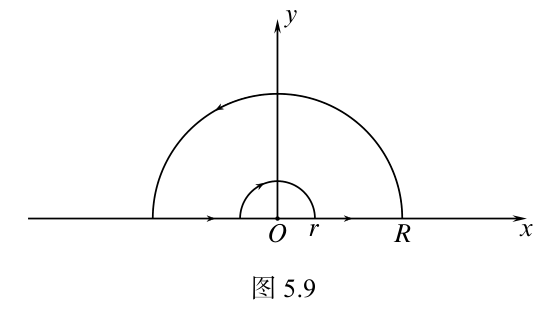
\includegraphics{public/figures/complex-functions/ch05-fig-5-9.png}

(11)
\(\displaystyle\int_0^\infty\frac{x^p}{1+x^2}\,dx=\frac{\pi}{2\cos(p\pi/2)}\)，\(-1<p<1\)。

(12)
\(\displaystyle\int_0^\infty\frac{x^p}{x^2+2x\cos\lambda+1}\,dx=\frac{\pi\sin(p\lambda)}{\sin(p\pi)\sin\lambda}\)，\(-1<p<1\)、\(-\pi<\lambda<\pi\)。

(13)
\(\displaystyle\int_0^\infty\frac{dx}{1+x^p}=\frac{\pi}{p\sin(\pi/p)}\)，\(p>1\)。

(14)
\(\displaystyle\int_{-\infty}^\infty\frac{e^{px}}{1+e^x}\,dx=\frac\pi{\sin\pi p}\)，\(0<p<1\)。

(15)
\(\displaystyle\int_0^1\frac{x^{1-p}(1-x)^p}{1+x^2}\,dx=\frac\pi{\sin\pi p}\left(2^{p/2}\cos\frac{p\pi}4-1\right)\)，\(-1<p<2\)。提示：对
\(z^{1-p}(1-z)^p/(1+z^2)\) 用图 5.10。

(16)
\(\displaystyle\int_0^1\frac1{(1+x)^2}\sqrt{\frac{(1-x)^3}{x}}\,dx=(1-\sqrt2/2)\pi\)。

(17)
\(\displaystyle\int_{-1}^1\frac{\sqrt[4]{(1-x)^3(1+x)}}{1+x^2}\,dx=(\sqrt{2+\sqrt2}-\sqrt2)\pi\)。

(18)
\(\displaystyle\int_0^\infty\frac{\log x}{x^2+2x+2}\,dx=\frac\pi8\log2\)。

(19)
\(\displaystyle\int_0^\infty\frac{\log^2x}{x^2+a^2}\,dx=\frac\pi{8a}(\pi^2+4\log^2a)\)，\(a>0\)。

(20)
\(\displaystyle\int_0^\infty\frac{\sqrt{x}\log x}{x^2+1}\,dx=\frac{\sqrt2\pi^2}{4}\)。

(21)
\(\displaystyle\int_0^\infty\frac{\log x}{x^2-1}\,dx=\pi^2/4\)。提示：对
\(\operatorname{Log} z/(z^2-1)\) 用图 5.11。

\noindent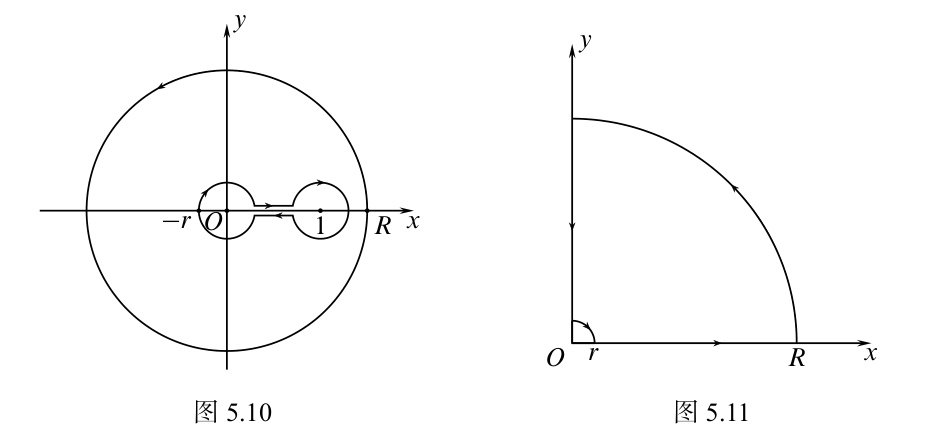
\includegraphics{public/figures/complex-functions/ch05-fig-5-10-11.png}

(22)
\(\displaystyle\int_0^1\frac1{x+1}\log\frac{1-x}{x}\,dx=\tfrac12\log^22\)。

(23) \(\displaystyle\int_0^\infty\log\frac{e^x+1}{e^x-1}\,dx=\pi^2/4\)。

(24)
\(\displaystyle\int_0^\infty\frac{\sin x}{e^x-1}\,dx=\frac\pi2\frac{e^{2\pi}+1}{e^{2\pi}-1}-\frac12\)。提示：对
\(e^{iz}/(e^z-1)\) 用图 5.12。

(25)
\(\displaystyle\int_0^\infty\frac{x}{e^x+1}\,dx=\pi^2/12\)。提示：对
\(z^2/(e^z+1)\) 用图 5.13。

\noindent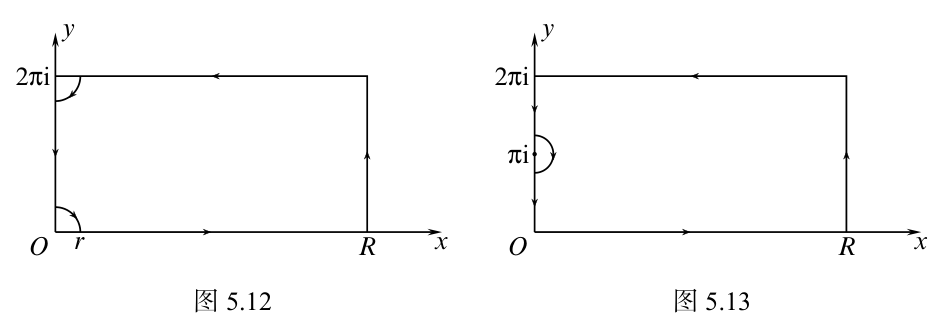
\includegraphics{public/figures/complex-functions/ch05-fig-5-12-13.png}

(26)
\(\displaystyle\int_0^\infty x^ne^{-x^{1/4}}\sin(x^{1/4})\,dx=0\)，\(n=0,1,2,\ldots\)。提示：对
\(z^{4n+3}e^{-z+iz}\) 用图 5.14。

(27)
\(\displaystyle\int_{-\infty}^\infty e^{-(x+ia)^2}\,dx=\sqrt\pi\)，\(a\in\mathbb R\)。

(28)
\(\displaystyle\int_0^\infty e^{-ax^2}\cos(bx^2)\,dx=\frac{\sqrt{2\pi}}4\sqrt{\frac{\sqrt{a^2+b^2}+a}{a^2+b^2}}\)，\(a>0\)。提示：对
\(e^{z^2(-a+ib)}\) 用图 5.15，角 \(\varphi\) 待定。

\noindent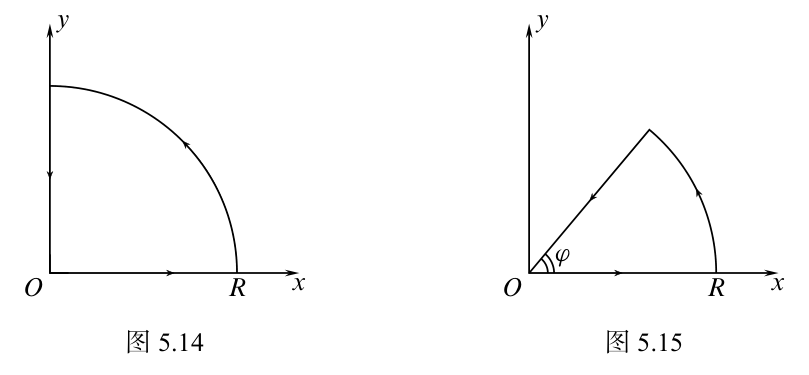
\includegraphics{public/figures/complex-functions/ch05-fig-5-14-15.png}

(29) \(\displaystyle\int_0^{\pi/2}\log\sin\theta\,d\theta\)。教材答案为
\(-\pi\log2\)（有误，见校注）。提示：先求广义积分
\(\int_0^{\pi/2}\log|e^{i\theta}-1|\,d\theta\)。

(30)
\(\displaystyle\int_0^\pi\frac{x\sin x}{1-2a\cos x+a^2}\,dx=\begin{cases}\frac\pi a\log(1+a),&0<a\le1,\\\frac\pi a\log(1+1/a),&a>1.\end{cases}\)
提示：对 \(z/(a-e^{-iz})\) 用图 5.16。

\noindent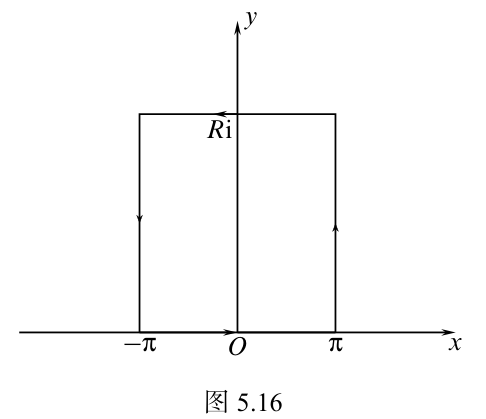
\includegraphics{public/figures/complex-functions/ch05-fig-5-16.png}

(31)
\(\displaystyle\int_0^\infty\frac{\log(1+x^2)}{1+x^2}\,dx=\pi\log2\)。

\par\Needspace{5\baselineskip}
\noindent\textbf{2.} 设 \(f\) 为有理函数，在 \([0,\infty)\)
上无极点，且无穷远点为其零点。证明：

\[
\int_0^\infty\frac{f(x)}{\log^2x+\pi^2}\,dx
=\sum_{k=1}^n\operatorname{Res}\left(\frac{f(z)}{\operatorname{Log} z-\pi i},a_k\right),
\]

其中取
\(\operatorname{Log} z=\log|z|+i\operatorname{Arg}z\)，\(0<\operatorname{Arg}z<2\pi\)。教材写``\(a_1=-1,a_2,\ldots,a_n\)
是 \(f\) 的全部不同极点''，按下述校注理解求和点集。

\subsubsection{本节校勘}\label{ch05-practice-ux672cux8282ux6821ux52d8-3}

第 1(12) 题在 \(p=0\) 或 \(\lambda=0\) 时右式按连续极限取值；第 1(15)
题在 \(p=0,1\) 同理。第 1(21) 题 \(x=1\)
是商的可去点，不必强行采用主值。第 1(29) 题正确答案为
\(-(\pi/2)\log2\)：记积分为 \(I\)，利用 \(\theta\mapsto\pi/2-\theta\)
后相加，再用 \(2\sin\theta\cos\theta=\sin2\theta\)，得
\(2I=I-(\pi/2)\log2\)。教材所给提示的积分区间也不能直接套用该答案。

第 2 题的求和点集应为 \(f\) 的全部有限极点与点 \(-1\)
的并集，重复点只计一次；因为 \(\operatorname{Log}(-1)=\pi i\)，即使
\(-1\) 不是 \(f\)
的极点，分母也会在那里产生零点。若奇点抵消，其残数为零。

\Needspace{5\baselineskip}
\subsection{习题 5.6}\label{ch05-practice-heading-6}

\par\Needspace{5\baselineskip}
\noindent\textbf{1.} 设 \(f,g\) 为域 \(D\)
上的亚纯函数，零点集、极点集及对应阶数均相同。证明存在 \(h\in H(D)\)，使
\(f/g=e^h\)。

\par\Needspace{5\baselineskip}
\noindent\textbf{2.} 设 \(a_n\) 在域 \(D\)
内互异且无聚点，\(\psi_n(z)=\sum_{j=1}^\infty c_{n,j}/(z-a_n)^j\) 在
\(D\setminus\{a_n\}\) 上全纯。证明存在
\(f\in H(D\setminus\{a_n:n\in\mathbb N\})\)，在每点 \(a_n\) 的 Laurent
主部恰为 \(\psi_n\)。

\par\Needspace{5\baselineskip}
\noindent\textbf{3.} 证明：\(f\) 在域 \(D\) 上亚纯，当且仅当有
\(g,h\in H(D)\)、\(h\not\equiv0\)，使 \(f=g/h\)。

\par\Needspace{5\baselineskip}
\noindent\textbf{4.} （插值定理的推广）设 \(a_n\) 在 \(D\)
内互异且无聚点，\(\varphi_n(z)=\sum_{j=-\infty}^\infty b_{n,j}(z-a_n)^j\)
在 \(D\setminus\{a_n\}\) 上全纯。证明：对任意整数列 \(k_n\)，存在
\(f\in H(D\setminus\{a_n:n\in\mathbb N\})\)，在 \(a_n\) 的 Laurent
展开为

\[
\sum_{j=-\infty}^{k_n}b_{n,j}(z-a_n)^j+\sum_{j=k_n+1}^\infty c_{n,j}(z-a_n)^j.
\]

\par\Needspace{5\baselineskip}
\noindent\textbf{5.} 设 \(a_1,a_2\in D\) 不同，Laurent 级数
\(\varphi_n(z)=\sum_{j=-\infty}^\infty b_{n,j}(z-a_n)^j\) 在
\(D\setminus\{a_n\}\) 全纯（\(n=1,2\)）。举例说明通常不存在
\(D\setminus\{a_1,a_2\}\) 上的全纯函数，其在两点的 Laurent 展开分别为
\(\varphi_1,\varphi_2\)。

\par\Needspace{5\baselineskip}
\noindent\textbf{6.} 证明 Weierstrass 因子分解定理对一般域成立。

\par\Needspace{5\baselineskip}
\noindent\textbf{7.} 证明插值定理对一般域成立。

\subsubsection{本节校勘}\label{ch05-practice-ux672cux8282ux6821ux52d8-4}

第 1 题在一般域上不成立，应补单连通条件，或改为要求无零全纯函数 \(f/g\)
的对数导数沿一切闭路的积分为零；反例是
\(D=\mathbb C\setminus\{0\}\)、\(f(z)=z\)、\(g(z)=1\)。还应排除恒零函数。第
4 题原式多出的右括号已去掉。第 6、7 题是教材正文中单连通版本的推广；讲义
§5.6 另给一般域补证，练习时应重建其中的因子构造，不能只援引单连通版本。

\Needspace{5\baselineskip}
\subsection{习题 5.7}\label{ch05-practice-heading-7}

\par\Needspace{5\baselineskip}
\noindent\textbf{1.} 用极点处 Laurent 主部表示下列亚纯函数：(1)
\(1/(e^z-1)\)；(2) \(1/\cos z\)；(3) \(\tan z\)；(4) \(1/\sin z-1/z\)。

\par\Needspace{5\baselineskip}
\noindent\textbf{2.} 将整函数进行因子分解：(1) \(e^z-1\)；(2)
\(e^{az}-e^{bz}\)；(3) \(\cos z\)；(4) \(\cos z-\sin z\)。

\par\Needspace{5\baselineskip}
\noindent\textbf{3.} 设 \(a_n\in B(0,R)\setminus\{0\}\)
互异，\(b_n=R^2/\overline{a_n}\)，\(k_n\in\mathbb N\)。证明：若
\(\sum k_n(R-|a_n|)<\infty\)，则
\(\prod_{j=1}^n[(z-a_j)/(z-b_j)]^{k_j}\)
在圆盘内闭一致收敛为到单位圆盘的全纯映射，零点恰为 \(a_n\)，阶数恰为
\(k_n\)。

\par\Needspace{5\baselineskip}
\noindent\textbf{4.} 设 \(a_n\in\mathbb C\setminus\{0\}\)
互异，\(k_n\in\mathbb N\)，且 \(\sum k_n/|a_n|<\infty\)。证明
\(\prod_{j=1}^n(1-z/a_j)^{k_j}\) 在平面内闭一致收敛为整函数，零点恰为
\(a_n\)，重数恰为 \(k_n\)。提示：考察 \(\sum k_n/(z-a_n)\)
的内闭一致收敛。

为紧凑书写以下原题，记
\(E_p(w)=(1-w)\exp(w+w^2/2+\cdots+w^p/p)\)，\(E_0(w)=1-w\)。

\par\Needspace{5\baselineskip}
\noindent\textbf{5.} 设 \(a_n\ne0\) 互异，\(k_n\in\mathbb N\)。证明：若存在
\(m\in\mathbb N\) 使 \(\sum k_n/|a_n|^{m+1}<\infty\)，则
\(\prod_{j=1}^nE_m(z/a_j)^{k_j}\)
在平面内闭一致收敛为整函数，零点与阶数恰为 \(a_n,k_n\)。提示：考察

\[
\sum_{n=1}^\infty k_n\left(\frac1{z-a_n}+\frac1{a_n}+\frac z{a_n^2}+\cdots+\frac{z^{m-1}}{a_n^m}\right).
\]

\par\Needspace{5\baselineskip}
\noindent\textbf{6.} 设 \(a_n\ne0\) 互异，\(k_n\in\mathbb N\)。证明：若有自然数列
\(p_n\)，使 \(\sum_{n=1}^\infty k_n(z/a_n)^{p_n+1}\)
在平面上绝对收敛，则 \(\prod_{j=1}^nE_{p_j}(z/a_j)^{k_j}\)
在平面内闭一致收敛为整函数，零点与阶数恰为 \(a_n,k_n\)。提示：考察

\[
\sum_{n=1}^\infty k_n\left(\frac1{z-a_n}+\frac1{a_n}+\frac z{a_n^2}+\cdots+\frac{z^{p_n-1}}{a_n^{p_n}}\right).
\]

\par\Needspace{5\baselineskip}
\noindent\textbf{7.} 设 \(a_n\ne0\)
互异，\(k_n\in\mathbb N\)，\(|a_n|\to\infty\)。证明
\(\prod_{j=1}^nE_{jk_j}(z/a_j)^{k_j}\)
在平面内闭一致收敛为整函数，零点与阶数恰为 \(a_n,k_n\)。

\par\Needspace{5\baselineskip}
\noindent\textbf{8.} 设 \(f\) 为非常数整函数，非零零点集为 \(a_n\)，相应重数为
\(k_n\)，\(k_0=\operatorname{Res}(f'/f,0)\)。证明有整函数 \(g\)，使

\[
f(z)=e^{g(z)}z^{k_0}\prod_{n=1}^\infty E_{nk_n}(z/a_n)^{k_n}.
\]

\par\Needspace{5\baselineskip}
\noindent\textbf{9.} 设有理函数 \(f\) 在无穷远点至少有二阶零点，全部不同极点
\(a_1,\ldots,a_m\) 均非整数。证明：

\[
\sum_{n=-\infty}^\infty f(n)=-\pi\sum_{k=1}^m\operatorname{Res}(f(z)\cot\pi z,a_k),\qquad
\sum_{n=-\infty}^\infty(-1)^nf(n)=-\pi\sum_{k=1}^m\operatorname{Res}(f(z)/\sin\pi z,a_k).
\]

\par\Needspace{5\baselineskip}
\noindent\textbf{10.} 求级数的和：

(1)
\(\sum_{n=-\infty}^\infty(a+n)^{-2}\)、\(\sum_{n=-\infty}^\infty(-1)^n(a+n)^{-2}\)，\(a\notin\mathbb Z\)；

(2)
\(\sum_{n=0}^\infty(n^2+a^2)^{-1}\)、\(\sum_{n=0}^\infty(-1)^n(n^2+a^2)^{-1}\)，\(a>0\)；

(3) \(\sum_{n=0}^\infty(-1)^n/(2n+1)^3\)；(4)
\(\sum_{n=1}^\infty n^{-2k}\)，\(k\in\mathbb N\)。

\par\Needspace{5\baselineskip}
\noindent\textbf{11.} 设 \(f\) 为 \(B(0,R)\) 上非常数的有界全纯函数，非零零点为
\(a_n\)，重数为 \(k_n\)。证明
\(\sum_{n=1}^\infty k_n(R-|a_n|)<\infty\)。

\par\Needspace{5\baselineskip}
\noindent\textbf{12.} 设 \(f\) 如第 11
题，\(k_0=\operatorname{Res}(f'/f,0)\)。证明有圆盘上无零点的有界全纯函数
\(g\)，使

\[
f(z)=g(z)z^{k_0}\prod_{n=1}^\infty
\left(\frac{R(a_n-z)}{R^2-\overline{a_n}z}\frac{|a_n|}{a_n}\right)^{k_n}.
\]

\subsubsection{本节校勘}\label{ch05-practice-ux672cux8282ux6821ux52d8-5}

第 2(2) 题 \(a=b\) 时函数恒零，应单独处理，通常的非零整函数因子分解需
\(a\ne b\)。第 6 题原求和下标写为 \(m\) 而项中用 \(n\)，已统一。第 8
题原指数二次项的系数印作 \(1/z\)，应为 \(1/2\)，本页用 \(E_p\)
统一展开式。第 8、11、12
题零点集可以有限或为空，相应乘积按有限乘积或空乘积理解；\(k_0\) 可为零。

\Needspace{5\baselineskip}
\subsection{习题索引}\label{ch05-practice-heading-8}

\hyperref[ch05-practice-heading-1]{习题 5.1} · \hyperref[ch05-practice-heading-2]{习题 5.2} ·
\hyperref[ch05-practice-heading-3]{习题 5.3} · \hyperref[ch05-practice-heading-4]{习题 5.4} ·
\hyperref[ch05-practice-heading-5]{习题 5.5} · \hyperref[ch05-practice-heading-6]{习题 5.6} ·
\hyperref[ch05-practice-heading-7]{习题 5.7}


\end{document}
